\documentclass[a4paper]{book}

\setlength{\parindent}{0ex}
\setlength{\parskip}{1.5ex}

\usepackage[dvips]{graphicx}
\usepackage{epsfig}
\usepackage{verbatim}

\usepackage[a4paper, hmargin=25mm, vmargin=30mm]{geometry}
\usepackage{syntonly}

\usepackage{ex201}
\usepackage{rex201}
\usepackage{styles201}
\usepackage{insn201}
%\syntaxonly

\title{COMP201 Reference}
\author{...}
\begin{document}

\maketitle
\tableofcontents


This manual is intended as an introduction to the REX boards equipped with WRAMP processors in Lab 1.
It's purpose is to get you started in programming for the WRAMP processor, and using the REX boards. It covers the basics of WRAMP assembly language, the WRAMP tools, as well as the I/O devices supplied on the REX boards.

It is designed to complement the lecture material of the COMP201 course.

Although every effort has been made to make this manual accurate, it is
possible that there may be errors in it.  If you find any please report
them to \emph{contact-cs201@cs.waikato.ac.nz}

This manual is mainly the product of a lot of hard work by Matt Jervis
and Jamie Curtis. Other people that have contributed to it's content
are Murray Pearson, Tony McGregor, and Dean Armstrong.


\chapter{Introduction}
\label{chapter:intro}
\section{Introducing the Basys3 and WRAMP}



This manual is intended as an introduction to WRAMPSys, which essentially 
comprises the Basys 3 boards with the FPGA programmed to perform as a WRAMP 
processor.  The manual includes information on programming for WRAMP and using 
the physical capabilities of the Basys boards. It covers the basics of the WRAMP 
assembly language, the WRAMP tools, and the I/O devices implemented on the 
Basys3 boards. Only the Basys3 itself is required for most of the
functionality, but the second serial port requires a Micro-USB PMOD expansion.
WRAMPsys can be used without this attached, but the second serial port will not function.

WRAMP is designed to be a simple architecture which can help you gain a practical
understanding of the internal workings of a computer. The initial implementation
on REX boards was developed at the University of Waikato by Dean Armstrong, as
part of an undergraduate degree. The implementation for Basys3 FPGAs was developed
by Daniel Oosterwijk and Tyler Marriner at the University of Waikato.

\subsection{The WRAMP CPU}
The \BI{Central Processing Unit} (\BI{CPU}) is responsible for carrying out 
instructions.
CPUs have developed at an astounding rate. From the humble Z80 to the 386, and
beyond the GHz barrier. But as the speed increases, so does
the complexity. Due to this complexity, it is difficult to learn to program
at a low level. 

The WRAMP CPU was designed to solve this problem. It is much easier to 
understand because it does not have the quirks of performance orientated CPUs.
Some features of the WRAMP CPU are:
\begin{itemize}
    \item An easy to understand instruction set. All instructions conform
            to a clear and consistent structure.
    \item All operations are carried out on 32-bit words.
    \item Only a single instruction is executed at a time.
    \item Memory addressing is easy to understand.
\end{itemize}

\subsection{The Basys board}
For a CPU to be usable, a motherboard is needed. Originally, the REX board was
developed to host the WRAMP CPU. However, the Basys FPGA can be reprogrammed
to take the form of both the WRAMP CPU and its peripheral components.
It should be connected via the Micro-USB port on the top-left to a Linux machine
with the \texttt{remote} tool installed.

The Basys board includes the following components:

\begin{description}
\item[CPU] The WRAMP processor is the brain of the Basys board.
%
\item[RAM] Capable of storing 16K words, the RAM resides at addresses 0x00000
to 0x03FFF. The last 2K words are reserved for use by the monitor program. The rest 
of the RAM is used to store and execute your programs, which, by default, are 
loaded starting from address 0x00000.
%
\item[ROM] Capable of storing 32K words, the ROM resides at addresses 
0x80000 to 0x87FFF. It is used to store the \WRAMPmon\ monitor program.
%
\item[Serial Interface] Allows the WRAMP processor to interface with two serial
ports. One is connected to a Linux machine via the Micro-USB port on the top-left
of the Basys board, which can also provide power. The other connects to the Micro-USB
port of a PMOD expansion, which should be connected to the bottom half of the 
top-left PMOD port.
%
\item[Parallel Interface] Allows the WRAMP processor to interface with: 
\begin{itemize}
\item a set of sixteen switches from which the CPU can read
\item three pushbuttons from which the CPU can read
\item four seven segment displays to which the CPU can write
\item a set of sixteen LEDs to which the CPU can write
\end{itemize}
\item[Timer] Counts down from a certain value and can interrupt the CPU when 
finished.
%
\end{description}
Use of these I/O devices will be covered in chapter \ref{chapter:io}.

\subsection{WRAMPmon}
The Basys board has installed on it monitor software known as \WRAMPmon.
It communicates with the user through the Linux machine connected to
the first serial port. \WRAMPmon\ is used to upload your programs to the
board and to debug them. This will be covered in more detail in
section \ref{intro:wrampmon}.
%
%
% SECTION - Assembly
%
\section{The WRAMP Assembly Language}
%
To help you get started we will begin by analysing, assembling,
executing and debugging a simple WRAMP assembly language program.
Using \program{emacs} (or your preferred text editor) enter the
program listed in Figure \ref{simple_prog}. Save it as \filename{intro.s}.
A digital copy is also bundled with this manual, named \filename{intro.s}.
You can simply use this to avoid retyping the program.

%%%
%
% Example Code
%
%%%
\begin{figure}[btp]
\begin{center}
%\begin{footnotesize}
\begin{tabular}{|p{15cm}|}
\hline
\begin{verbatim}
 .text
 .global main
 main:
      # Get the address of the welcome message
      la     $2, welcome_msg
      # Display the message
      jal    putstr
      # Clear our sum register
      add    $4, $0, $0
      # Initialise the loop counter
      addi   $5, $0, 1
 loop:
      # Read a number from the user
      jal    readnum
      # Add it to our running total
      add    $4, $4, $1
      # Increment our loop counter
      addi   $5, $5, 1
      # Test to see if we have done all 4 numbers
      slti   $1, $5, 4
      # Keep looping until 4 numbers have been entered
      bnez   $1, loop
      # Get the output message
      la     $2, output_msg
      # Print it
      jal    putstr
      # Move our sum into register $2 to display it
      add    $2, $0, $4
      # Print out the number
      jal    writenum
      # Return to the monitor
      j      exit
 .data
      # This is our welcome message
 welcome_msg:
      .asciiz  "Welcome to the world of WRAMP!!!\n\nPlease
               type four numbers, pressing enter after each:\n"
      # This is the output message
 output_msg:
      .asciiz    "The sum of the numbers is : "
\end{verbatim}%$

\\
\hline
\end{tabular}
%\end{footnotesize}
\end{center}
\caption{WRAMP Assembly Language Program (\filename{intro.s})}
\label{simple_prog}
\end{figure}
%%%%
%%%
%%
%

This program first displays a message asking you to enter four numbers. It
is then meant to input four numbers, add them up and display the result. 
If you have noticed the bug in it, don't worry as we will correct this later.

As you read through the source file look for the following:

\begin{description}
\item[comments] are lines beginning with a hash (\src{\#}). These work in
the same way as \src{//} comments in C and are ignored by the assembler.
%
\item[labels] such as \src{main:} are used to refer to a location in the
memory. This may be used to move execution to a different area of code or
to refer to data in the memory.
%
\item[directives] are commands beginning with a period (\src{.}). They
pass information to the assembler.
%
\item[subroutine calls] are used in this program to perform hardware
operations such as reading from the serial port. For example the
lines \src{jal putstr} and \src{jal readnum} are subroutine calls.
%
\item[WRAMP instructions] such as \src{add \reg{4}, \reg{0}, \reg{0}} get
converted to machine code by the assembler. They can then be executed by the
WRAMP CPU.
%
\end{description}

\subsection{Labels}
A label is a means of referencing a location in memory. Rather than
specifying absolute addresses when accessing data in memory, a label
can be used. This makes it much easier for the programmer to write
and understand the code. Labels can also be declared within the
code. They can then be used as a destination for branch and jump
instructions.

A label declaration consists of a name (containing no spaces) followed
by a colon (\src{:}). A label name can include alphanumeric characters,
underscores (\src{\_}), and periods (\src{.}).

The example code in figure \ref{simple_prog} has labels \src{main},
\src{loop}, \src{welcome\_msg}, \src{output\_msg}. The labels
\src{main} and \src{loop} refer to locations within the code. The
labels \src{welcome\_msg} and \src{output\_msg} refer to data.

In addition to any labels declared by the user, three special labels
can be used: \src{text\_size}, \src{data\_size}, and \src{bss\_size}.
These labels will resolve to the size of each section of the program:
for example, \src{text\_size} will be the number of instructions
in the \src{.text} section. These sections are discussed below.

\subsection{Directives}
Directives (commands preceded by a \src{.}) do not become part of the
final executable. They are used to pass information to the assembler,
like \src{\#} directives do in C.

\subsubsection{\text, \data and \bss}
A program written in WRAMP assembly can be split into three sections.
These are used to separate executable code, initialised data, and
uninitialised data. The directives \text, \data and \bss are used to
do this. When the assembler encounters one of these directives it
knows that all the code following it belongs in the given section.

The \text section contains WRAMP assembly instructions which will be
converted to machine language which can be executed on the WRAMP CPU.

%The \data section is used for initialised data.
Within the \data section, space in the memory can be reserved and
initialised. This is useful for strings, constants, and variables
which have an initial value.

The \bss section allows memory space to be reserved but not initialised.
The advantage of this is that space can be reserved in chunks using a single
command. This feature makes the \bss section useful for arrays.

\subsubsection{Assigning Space}
Within the \data and \bss sections, memory space is assigned using directives. 
To be able to access this you need to place a label before the assigning
directive. In the example code, the label \src{welcome\_msg:} refers to the
memory reserved by the \asciiz directive.

\begin{verbatim}
   welcome_msg:
      .asciiz "Welcome to the world of WRAMP!!!\n\n"
\end{verbatim}

The following is a list of the available memory assigning directives
and how they can be used.

\begin{description}

\item[\word \src{n}] assigns one word of memory space and initialises it to
the number \src{n}.
If a character is provided instead of a number, like \src{\word `a'}, the space
will be initialised to the ASCII value of that character.
If the name of a label is provided, like \src{\word main}, the space will be
initialised to the address of that label.

\item[\asciiz \src{"str"}] reserves and initialises space 
for a NULL terminated ASCII string (\src{"str"}).
This means that the string is followed immediately by a NULL
character (\src{0}). The NULL character can then be used
to identify the end of the string.

\item[\ascii \src{"str"}] reserves and initialises space for 
the ASCII string \src{"str"} without NULL terminating.

\item[\Space \src{n}] is used to allocate a chunk of space 
of size \src{n} in the \bss section.

\end{description}

The \ascii and \asciiz directives cannot be used in the \bss section
as they initialise the space they reserve. The \word directive may be
used as long as it is not provided with an argument.

\subsubsection{Escape Characters}

Any string or character literal can include some special characters which
are otherwise difficult to type. The following is a list of the valid
escape sequences and their uses.

\begin{description}

\item[\src{\textbackslash r}] is the `carriage return' character, which moves
the cursor back to the start of the current row.

\item[\src{\textbackslash n}] represents the `newline' character, which moves the
cursor down one row. If combined with a carriage return, like
\src{"\textbackslash r\textbackslash n"}, the cursor moves to the beginning of the next line.

\item[\src{\textbackslash t}] is a tab character. When this is printed directly to
the serial port, the cursor will move to the next point in the current
row whose index is a multiple of 8. This is similar to setting the
tab width to 8 in any common text editor.

\item[\src{\textbackslash a}] is the bell character. Printing this character
will cause your terminal's bell to ring, which may be audible or visual
depending on your settings.

\item [\src{\textbackslash\textbackslash}, \src{\textbackslash'},] and
\src{\textbackslash"} will produce a literal \src{\textbackslash},
\src{\char13}, and \src{"} respectively.

\item[\src{\textbackslash 0}] allows you to enter arbitrary escape sequences.
Any numeric characters immediately following this are read as an octal value,
and the ASCII character code they represent is placed in the string. Note that
the result will be truncated to the least significant 8 bits, and that any 8s
or 9s in the sequence may produce unexpected behaviour. Many ASCII reference
tables, such as \src{man 7 ascii}, show octal representations to make writing
these easier.

A particularly useful escape sequence is \src{\textbackslash 033}. Printing
the control sequence \src{"\textbackslash 033[yy;xxH"} will cause the cursor
to move to the location referenced by \src{yy} and \src{xx} (yy being row
count, and xx being column count). These numbers are 1-indexed and decimal.
For example, the following text is printed at the top-left corner of the
screen:

\begin{verbatim}
   Hello world!
\end{verbatim}

To change this to \src{Hello WRAMP!} without reprinting the parts of the string
which do not need changing, the following sequence could be printed:

\begin{verbatim}
   \033[01;07HWRAMP
\end{verbatim}

A selection of other standard VT100 terminal control codes are supported by
\program{remote}. There is no full list of which of these control codes
\program{remote} supports, but the list of standard control codes can be found
online.

\end{description}

\subsubsection{The \Global Directive}
When linking multiple files, we need to share functions and data.
However, we do not want to expose all the labels in a file.
Only labels declared as global (using the \Global directive) are
accessible outside the current file.

In the example program, we have declared the `entry point' \src{main}
as global. To do this we used the following directive:
\begin{verbatim}
   .global main
\end{verbatim}

\subsubsection{The \equ Directive}
When writing large programs, it can be useful to declare a number of
constants to avoid the use of magic numbers. The \equ directive will
create a named constant, which is simply an alias to a number. It is
similar to a \src{\#define} directive in C. It will not define an
area in memory, nor will it exist in a compiled program aside from
where it is used. The directive can be used as follows:

\begin{verbatim}
   .global main
   .text
   main:
      lw $1, switches($0)
      sw $1, leds($0)
      j main

      .equ   switches, 0x73000
      .equ   leds,     0x7300A
\end{verbatim}

This creates a program which will continually read from the switches
and save their value to the LEDs. It has no reserved memory.

\subsection{Registers}
Registers are the CPU's equivalent of variables. There are 16 general
purpose registers numbered 0 to 15. They can be used for temporarily
storing data while it is used in operations. Registers are generally
referred to by a \$-sign followed by a number. For example \reg{0}
refers to register zero. The contents of registers can be transferred
to and from main memory. This done using load and store instructions,
which are covered in a later section.

Some of the general purpose registers have special uses:

Register \reg{0} is always zero. Any attempts to write to it are
ignored. This provides a constant source of zero that can be used for
comparing and initialising registers.

Register fourteen is denoted \reg{sp}. This register is defined by
convention to be the stack pointer. While the hardware imposes no
special conditions on this register, failure to follow this convention
may affect the ability of code to interoperate with other software.

Register fifteen is denoted \reg{ra}. It is defined by convention to
be the subroutine return address register. When a jump and link
instruction is executed, this register is loaded with the address of
the next instruction after the jump and link. We will discuss stacks
and this register in a later chapter.

In addition to these general purpose registers is a set of special
purpose registers. The use of these is covered in chapter
\ref{chapter:exceptions}.

Various types of instructions are introduced below.

\subsection{Instructions}

Executable machine code is created by assembling WRAMP instructions.
Instructions tell the WRAMP CPU what to do. For example an \src{add}
instruction will add the contents of two registers and place the result
in another.

\subsubsection{Arithmetic}
Arithmetic instructions come in four forms, which are listed
below, using \src{add} as an example:


\src{add \regd, \regs, \regt} \\*
Simply performs the specified operation
on \regs\ and \regt, placing the result in \regd. For example,
\mbox{\src{add \reg{1}, \reg{2}, \reg{0}}} will add the contents of registers
\reg{2} and \reg{0} then place the result in \reg{1}.
\\

\src{addi \regd, \regs, Immediate} \\*
This is known as immediate form.
The argument \src{Immediate} is a constant. Thus the specified
operation is performed on \regs\ and \src{Immediate}, and the result
placed in \regd. For example \mbox{\src{addi \reg{1}, \reg{2}, 4}} will add
\src{4}\ to the contents of \reg{2}\ and place the result in \reg{1}.
Keep in mind that \src{Immediate} is a sign extended 16-bit twos compliment integer,
meaning the range of numbers is \src{-32,768} to \src{32,767}.
\\

\src{addu \regd, \regs, \regd} \\* 
The \emph{u}\ tells the CPU that this is an unsigned instruction.
Both operands will be treated as positive, which is important when
we consider the two's complement representation of negative numbers.
For example, \mbox{\src{1111 1111 1111 1111 1111 1111 1111 1111}} 
represents \src{-1} when treated as signed, and 0xFFFFFFFF, a very 
large positive number, when treated as unsigned.
\\

\src{addui \regd, \regs, Immediate} \\*
This is the combination of the two forms above. It performs an unsigned
operation on \regs\ and the \src{Immediate} value.
\\

For a full listing of arithmetic instructions see Appendix
\ref{appendix:instr}.

\subsubsection{Memory I/O}
The WRAMP CPU has a 20-bit memory space. Of this, the memory locations 
0x00000 to 0x03FFF are RAM.

Unlike other CPUs, WRAMP has only a single method of referencing
external memory. It consists of a base address added to an offset.
The base address is specified as a constant in the instruction. The
offset is the contents of a specified register.

The notation for this is \src{base(\regs)}. The \src{base} can either
be a label or an integer. To load from the memory location specified
by a label, \reg{0} can be used for \regs. We will mostly use this method
of accessing memory. Figure \ref{memio} shows an example.
It loads a word of data from memory into a register, adds 1 to it,
then stores it back into the memory.

\src{lw \regd, base(\regs)}\\*
Used to get the contents of the specified memory location and place it 
in the register \regd.

\src{sw \regd, base(\regs)}\\*
Will place the contents of \regd\ into the specified memory location.

As well as the \src{base}, a constant offset can also be provided to
\src{lw} and \src{sw} instructions:

\src{lw \regd, base+1(\regs)}\\*
This will load from the address directly after the one pointed to by
\src{base}. A negative offset can also be provided, such as \src{base-1}.
This allows a user to do things like indexing directly to a constant
offset in an array. Care must be taken to not provide an offset that
points to an unexpected memory location, especially when using negative
offsets.

\begin{figure}[btp]
\begin{center}
%\begin{footnotesize}
\begin{tabular}{|p{15cm}|}
\hline
\begin{verbatim}
.text
     . . .

     #Read from the memory location `counter' into $4
     lw $4, counter($0)

     #Add 1 to $4
     addi $4, $4, 1

     #Store the contents of $4 into the memory location `counter'
     sw $4, counter($0)

     . . .
     
.data
     # This is our counter
counter:
     .word 0 
\end{verbatim}%$
\\
\hline
\end{tabular}
%\end{footnotesize}
\end{center}
\caption{Memory I/O Example}
\label{memio}
\end{figure}

Sometimes you will need to know the address of a variable. The 
instruction `load address' ( \src{la} ) is used for this. It has the 
structure:

\src{la \regd, label} \\*
Load the address that \src{label} refers to into register \regd.
This instruction also allows loading of a 20 bit immediate to a register.
This instruction is also the method used to use the special labels 
\src{text\_size}, \src{bss\_size}, and \src{data\_size}.

\subsubsection{Test Instructions}
These instructions are used to compare either two registers, or a
register and an immediate value. They take the same form as
arithmetic instructions. If the test passes the destination register
is set to \src{1}, otherwise, it is cleared to \src{0}.

For example, to test if registers \reg{2} and \reg{3} were equal and store the
result in \reg{1} we would use the `set if equal' instruction: 
\src{seq \reg{1}, \reg{2}, \reg{3}}.

A full listing of test instructions can be found in the instruction set reference, Appendix \ref{appendix:instr}.

\subsubsection{Program Control}
We can move execution to a different part of the program using two types
of instruction: the unconditional jump, and the conditional branch.

\textbf{Jump Instructions}\\*
The jump instructions simply move execution to a different line of
code. They are unconditional and so do not perform any tests first.
There are four different varieties:

\src{j label} - Jump\\*
Jumps to the specified label.

\src{jal label} - Jump and link\\*
Stores the address of the next instruction into the return address register
\reg{ra}. It then jumps to the specified label. This is used when calling
subroutines.

\src{jr \regs} - Jump Register\\*
Jumps to the location specified by the contents of the register \regs.
Because the WRAMP CPU has only a 20-bit address space the upper 12 bits
of the register are ignored. Jump register is typically used to
return from a subroutine using \src{jr \reg{ra}}

\src{jalr \regs} - Jump and Link Register\\* 
A combination of \src{jal} and \src{jr}. 
It works in the same way as \src{jr}, but it stores the address of the
next instruction into the return address register before jumping.

\textbf{Branch Instructions}\\*
Branching instructions are conditional. They look at whether a
register is zero or not and act on that information. There are two
varieties: `branch if equal to zero' \src{beqz} and `branch if not
equal to zero' \src{bnez}. Both of these instructions take a single
register and a label as arguments.

For example the `branch if not equal to zero' command
\src{bnez \reg{1}, loop} will branch to label \src{loop} if
\reg{1} is non-zero.

\subsection{Assembling and Linking}
Before we can execute our program on the Basys board we need to
translate it into machine code, so that the WRAMP CPU can understand it.
This is a two-step process.

Please see Appendix \ref{appendix:wasm-wlink} for additional details
on the usage of these tools, as well as some supplementary tools.

\subsubsection{Assembly}
First, we have to \BI{assemble} the source code using a program
called an \filename{assembler}. This involves checking that all the
directives and instructions within the program make sense (are
syntactically correct). The program is then translated into a file
called an \BI{object file}. This contains portions of machine code
along with other information about the program.

To assemble our file we use the WRAMP \BI{assembler}, \program{wasm}:
\begin{verbatim}
   wasm intro.s
\end{verbatim}

There should now exist a file called \filename{intro.o}. This is the 
\BI{object file}. You can manually specify a filename by providing the
\src{-o} flag, but the default name is usually the clearest: the
object file created from the source file with the same name.

\begin{verbatim}
   wasm -o intro.o intro.s
\end{verbatim}

\subsubsection{Linking}
Next we must \BI{link} the \BI{object file}. A program may be
comprised of many separate parts. Even our example program contains
functions (subroutines) contained in a separate \BI{library}. Linking
involves joining all these parts together to create a final program.

The WRAMP \BI{linker} is called \program{wlink}. We will use it to
link our object file to the library object file bundled with this manual.
Issue the command:
\begin{verbatim}
     wlink -o intro.srec intro.o lib_manual.o
\end{verbatim}

This command links together the object files to create a file called
\filename{intro.srec}. This file is in a form known as S-Record, which
is suitable to be uploaded to WRAMPmon and executed.

%
%
% SECTION - WRAMPmon
%
\section{Introduction to WRAMPmon}
\label{intro:wrampmon}

The \WRAMPmon\ monitor is a program which runs on the Basys boards. It
provides you with basic facilities for interacting with the board.
It is important for hardware and software development, debugging,
testing and troubleshooting. It uses a command line interface to
perform these functions.

\WRAMPmon\ communicates through the first serial port, which is usually
connected to a Linux machine.
By running a terminal emulator on the Linux machine, we can talk to the board.

\subsection{WRAMPmon commands}
A set of commands is provided for the user to interact with \WRAMPmon\
including:

\begin{itemize}
\item a help command (\src{help}, or \src{?})
\item commands to view and alter the memory and register contents
\item a command to upload your programs
\item commands to execute programs in the memory
\item commands for debugging
\end{itemize}

For a listing of these commands see Appendix \ref{appendix:wrampmon}.

\subsection{Getting started}
The Basys board uses serial ports as its primary form of communication.
The first serial port on the board should be connected to a Linux
machine. The Linux machine runs a terminal program, called
\filename{remote}, which transmits anything typed on the keyboard
directly to the board, and displays any text received from WRAMP.

To execute the terminal program type \src{remote} from a console.
Once you have \src{remote} running you will need to reset the
board by pressing the \src{RESET} button, the \src{RESET} button is the
top button in the group of 5. 
You should see something like Figure \ref{wrampmon}.

\begin{figure}[h]
\begin{center}
\begin{tabular}{|p{15cm}|}
\hline
\begin{verbatim}
      +------------------------------------------------+
      |                 WRAMPmon 0.7                   |
      | Copyright 2002, 2003 The University of Waikato |
      |                                                |
      |          Written by Dean Armstrong             |
      |       Ported to the Basys3 in 2018 by          |
      |     Daniel Oosterwijk and Tyler Marriner       |
      +------------------------------------------------+
      
      Type ? and press enter for available commands.
      
       > 
\end{verbatim}
\\
\hline
\end{tabular}
\end{center}

\caption{\WRAMPmon}
\label{wrampmon}
\end{figure}

Type \src{?} to obtain a list of commands available within \WRAMPmon.

Help on individual commands can be obtained by typing the command and then a 
question mark, eg:
\begin{verbatim}
   load ?
\end{verbatim}

Each command gives the required format and available options.
An item enclosed in square brackets, \src{[}~and~\src{]},
indicates an optional item. An item enclosed in angled brackets, 
\src{<}~and~\src{>}, indicates a compulsory item.

If you have any problems with the monitor not responding at any stage you 
should always be able to get back to the board's initial state with the
start-up message displayed by pressing the \src{RESET} button.

\subsection{Uploading and Executing your Program}
Before you can run your program on the Basys board it must first be loaded
into the board's memory. This can be done by setting the board into \src{load}
mode and using the upload option within the \program{remote} program to send
the S-Record file from the Linux machine to the board. To place the board
into load mode, type the following command (then press enter) at the
\WRAMPmon\ prompt:
\begin{verbatim}
   load
\end{verbatim}

After hitting return there should be a reminder response from the board
indicating how to send an executable file. To send the executable type:

\verb|   <ctrl>-a| and then \verb|s|

Where \verb|<ctrl>-a| means press and hold the \src{control} key, hit 
the \src{a} key and then release both keys.
The \program{remote} program does not pass this key sequence on to the Basys 
board but instead enters a command mode. When you press \src{s}, remote will
switch into upload mode. A dialogue box appears which asks you to enter the name
of the file you wish to upload. Type in the following file name:
\begin{verbatim}
   intro.srec
\end{verbatim}

After the file name has been entered a series of dots should appear on the 
screen indicating that the file is being uploaded, followed by a message which
tells you that is has completed. You should then press the enter key to
leave the upload mode of \src{remote} at which stage the \WRAMPmon\ prompt 
should reappear.

If any characters which are not dots appear, it means that \WRAMPmon\ did not
correctly receive the program data. \program{remote} will try again until it
reaches ten failures. If this happens, you should check the connection between
the Linux machine and the Basys board, and recompile the S-Record file.

Now that the program has been uploaded, you can run it by typing the command:
\begin{verbatim}
   go
\end{verbatim}

This will start executing your program from the entry point defined by the 
\src{main} label. The program will prompt you to enter four numbers. You
should continue to type a number and hit enter until the program outputs the
resulting sum. The output of your program should appear on your screen. When
the \WRAMPmon\ prompt appears again it indicates that your program has finished
executing.

\subsection{Debugging your Program}
\label{intro:debugging}
The program that you have just run on the Basys board should have read four
numbers from the keyboard and output their sum to the terminal. However, when
run, only three numbers are read before their sum is output.

In this section of the exercise, you are going to use the debugging 
features of \WRAMPmon\ to locate the bug that causes this problem.

The debugging commands within \WRAMPmon\ allow you to trace the execution 
of a program (i.e. follow the path of execution) by inserting breakpoints.

If a breakpoint is set at a certain instruction, then when the program
is running, and that instruction is about to be executed, control will
be returned to the monitor. From here, you can view register and
memory contents, and maybe resume execution, or step through the
program one instruction at a time to try and identify bugs. The
commands for setting, removing and viewing breakpoints are \src{sb},
\src{rb}, and \src{vb} respectively. The help functions in \WRAMPmon\
fully describe the operation of these commands. For example, to find
out more about the set breakpoint command type
\begin{verbatim}
   sb ?
\end{verbatim}

Insert a breakpoint at the beginning of the loop in the above program 
(ie. at memory location \src{0x00004}), and execute the program using
the \src{go} command.
When a break does occur, use the view registers command to find out 
the contents of the registers. You should also notice that the breakpoint 
register dump contains identical information to the \src{vr} command.

To continue execution type:
\begin{verbatim}
   cont
\end{verbatim}
This will cause the program to continue execution until either the
breakpoint is encountered again or the program completes execution.
Remember that the program will now wait for you to enter a number
before it will break again.

Another feature of the monitor that can be used to help debug your programs
is the single-step command \src{s}. This command causes only the
immediately next instruction to be executed, then returns back to
\WRAMPmon.

To demonstrate the use of the single step command, you should reset the
board and reload the program. Create a new breakpoint at memory location
\src{0x00005}. Once this is done run the program using the \src{go}
command.

Once you have encountered the breakpoint, try single stepping through
the program using the \verb|s| command. Pay careful attention to the
loop counter in \reg{5} and the instructions that increment and test
that register. As we are only interested in the loop counter at this
stage we will skip the \src{readnum} subroutine. We can do this using
the `step over' \src{so} command. When you reach the instruction \src{jal
readnum} type `\src{so}' instead of `\src{s}'.

At some point, you may wish to remove the breakpoint using the
\src{rb} command and then use \src{cont} to make the program run to
completion.

As you may have noticed, the program is designed with a bug. Although
it is intended to add 4 numbers, it will only add 3. You should now use
the debugging methods we have just covered to determine the cause of the
bug. Correct it then and assemble, link, and load the program to confirm
it now operates correctly.

\chapter{Stack Guide}
\label{chapter:stack}
%%
%
% Body
%
%%
\section{WRAMP Stack Frame}

A stack is a term used to describe a `first in, last out' buffer. New
items are placed on the top of the stack, and must be removed before
older items. Two terms are commonly used to refer to the operations of
adding to, and removing values from a stack. A push operation puts a
new value at the very top of the stack, and a pop operation removes the
item from the top of the stack. These are the only operations allowed to
be performed on a stack, and there is no way to remove an older item
before a newer one. Stacks provide an ideal mechanism for passing
parameters to a function and providing storage for local variables and
temporary results inside a function. This document describes the
reasons a stack is used on the WRAMP architecture, how the stack is
created, and the conventions surrounding its use.

The WRAMP processor itself does not directly support a stack, but
it is possible to setup a stack in software. To achieve this, a block
of memory for the stack to reside in must be set aside. On the Basys
board, \WRAMPmon\ does this for you. The stack starts at the top of
memory, with new items placed at lower memory addresses. Because of
this, stacks on the WRAMP architecture are often referred to as
growing downwards.

%%%
%
% PUSH FIGURE
%
%%%
\begin{figure}[!hb]
\begin{center}
\begin{footnotesize}
\begin{tabular}{|c|c|c|}

\hline
%% Text....
\begin{minipage}[l]{7cm}
\vspace{\topsep}
\begin{verbatim}

push:
      # move the stack pointer down
      # by one to create space for 
      # a value to be pushed onto 
      # the stack.

      subui $sp, $sp, 1

      # store the contents of $2 onto
      # the new space on the stack

      sw $2, 0($sp)

\end{verbatim}
\end{minipage}
&
%% Fig before
\begin{minipage}[c]{3.5cm}
\begin{center}
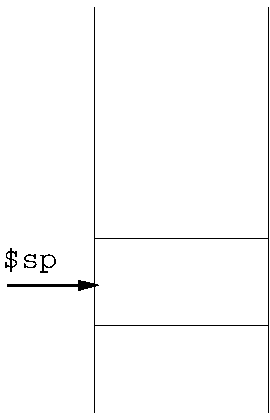
\includegraphics[width=2.2cm]{stack_fig1_a.eps}
%\vspace{0.1cm}

\emph{before}\\
\end{center}
\end{minipage}

&
%% Fig after
\begin{minipage}[c]{3.5cm}
\begin{center}
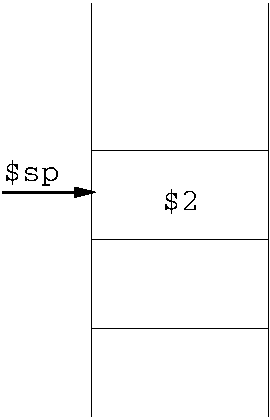
\includegraphics[width=2.2cm]{stack_fig1_b.eps}


\emph{after}\\
\end{center}
\end{minipage}
\\
\hline
\end{tabular}
\begin{center}
\small{
\textbf{(a) WRAMP code}
\hspace{3.5cm}
\textbf{(b) Stack Diagrams}
}
\end{center}

\caption{Push}
\label{fig:stack_push}
\end{footnotesize}
\end{center}
\end{figure}
%%%
%
% End of PUSH figure
%
%%%

To place new items onto and remove existing items from the stack you
need a way to know the current address of the top of the stack. To
allow this, a register is set aside to store this address. This
register is referred to as the ``top of stack'' pointer, or more often
just the ``stack pointer''. By WRAMP convention, the stack pointer is stored
in register 14 and is referred to as \src{\$sp} in WRAMP assembly code.
Figure \ref{fig:stack_push}(a) shows example WRAMP code to ``push'' a new
value onto the stack and (b) shows the stack before and after the push operation. Figure \ref{fig:stack_pop} shows the WRAMP code and stack diagrams for a pop
operation.

%%%
%
% POP FIGURE
%
%%%
\begin{figure}[!ht]
\begin{center}
\begin{footnotesize}
\begin{tabular}{|c|c|c|}

\hline
%% Text....
\begin{minipage}[l]{7cm}
\vspace{\topsep}
\begin{verbatim}

pop:
      # pop into register 3 the value
      # stored on the top of the
      # stack

      lw $3, 0($sp)

      # Move the stack pointer up
      # by one to remove item

      addui $sp, $sp, 1

\end{verbatim}
\end{minipage}
&
%% Fig before
\begin{minipage}[c]{3.5cm}
\begin{center}
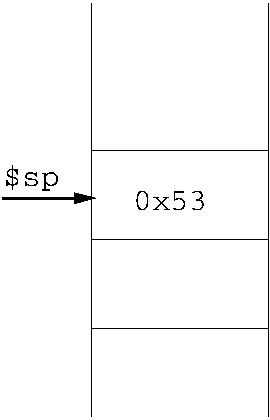
\includegraphics[width=2.2cm]{stack_fig2_a.eps}
%\vspace{0.3cm}

\emph{before}\\
\end{center}
\end{minipage}

&
%% Fig after
\begin{minipage}[c]{3.5cm}
\begin{center}
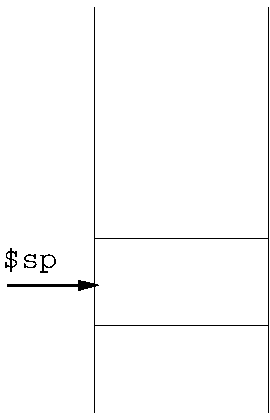
\includegraphics[width=2.2cm]{stack_fig2_b.eps}

%\vspace{0.3cm}
\emph{after}\\
\end{center}
\end{minipage}
\\
\hline
\end{tabular}
\begin{center}
\small{
\textbf{(a) WRAMP code}
\hspace{3.5cm}
\textbf{(b) Stack Diagrams}
}
\end{center}

\caption{Pop}
\label{fig:stack_pop}
\end{footnotesize}
\end{center}
\end{figure}
%%%
%
% End of POP figure
%
%%%
\vspace{0.2cm} %Push to the next page

\section{WRAMP Stack Conventions}
On the WRAMP architecture the stack is used to:

\begin{itemize}
\item store local variables that are not stored in registers
\item temporarily store the contents of registers so that a subroutine can use them while making sure the previous contents are preserved.
\item pass parameters to a subroutine
\end{itemize}

%%%
%
% Figure 3
%
%%%
\begin{figure}[!hbt]
\begin{footnotesize}
\begin{center}
\begin{tabular}{|p{10cm}|}
\hline
\begin{verbatim}
parent:
       addi $3, $0, 5
loop:
       beqz $3, endloop
        ...
       jal child
        ...
       subi $3, $3, 1
       j loop

endloop:
       j exit

child:
        ...
       add $3, $4, $5
        ...
       jr $ra
\end{verbatim}
\\
\hline
\end{tabular}
\end{center}
\end{footnotesize}
\caption{Incorrect Function} 
\label{fig:problemcode}
\end{figure}

\section{Saving Registers}
When a program contains a number of subroutines that can call each
other, a set of conventions is required to ensure that a subroutine
does not use a register and modify values that a parent subroutine is
also using. For example consider the code sequence in Figure
\ref{fig:problemcode}. Notice that the section of code labelled
\src{parent} is using \src{\$3} as a loop counter that decrements each
time through the loop. Inside this loop is a call to the subroutine
\src{child} that uses \src{\$3} to store an intermediate result. This
would overwrite the loop counter value stored in that register by the
subroutine \src{parent}. While it would be possible in this simple
sequence to rearrange the code to fix the problem, it will not always
be possible to do so. To ensure problems like this do not occur in
code there needs to be a set of conventions controlling the way
registers are used.

The convention used in the WRAMP architecture is that all subroutines
must save the contents of a register to the stack before it can use
it. The value must then be restored from the stack before the
subroutine exits. It should be noted that it is up to the programmer
to ensure these conventions are followed and the processor does not
enforce them in any way. For code generated by a C compiler, the
compiler must ensure that these same conventions are followed. Figure
\ref{fig:correctcode} shows the corrected program that follows the
conventions.

When a subroutine is called using the \src{jal} instruction, the
return address for the subroutine is placed in register 15
(\src{\$ra}). If this subroutine then uses \src{jal} to call another
subroutine it will overwrite its own return address. Because of this,
any subroutine that is going to call another subroutine needs to save
\src{\$ra} onto the stack before calling the routine and restore it
before it returns. Figure \ref{savera} gives an example of this.


%%
%
% Figure 4
%
%%%
\begin{figure}[!hb]
\begin{footnotesize}
\begin{center}
\begin{tabular}{|p{10cm}|}
\hline
\begin{verbatim}
parent:
       addi  $3, $0, 5
loop:
       beqz  $3, endloop
        ...
       jal   child
        ...
       subi  $3, $3, 1
       j     loop

endloop:
       j exit

child:
        ...
       # save register 3 before we overwrite
       # the contents of it
       subui $sp, $sp, 1
       sw    $3, 0($sp)

       add   $3, $4, $5
        ...
       # restore the old contents of register
       # 3 before we return
       lw    $3, 0($sp)
       addui $sp, $sp, 1

       jr    $ra
\end{verbatim}
\\
\hline
\end{tabular}
\end{center}
\end{footnotesize}
\caption{Correct Function}
\label{fig:correctcode}
\end{figure}

There is one exception to the rule that all registers must be
saved. For reasons discussed in the next section, register 1
(\src{\$1}) never needs to be saved or restored.

\section{Parameter Passing}
In Chapter \ref{chapter:intro}, parameters were passed to
subroutines using regsiters. While this works in this simple case
consider what would happen if a subroutine required a large number of
parameters or called other subroutines. It is not difficult to see that
with a large program it would not take long to exhaust the registers
available to the programmer on the WRAMP processor.

%%%
%
% Figure 5
%
%%%
\begin{figure}[!htbp]
\begin{footnotesize}
\begin{center}
\begin{tabular}{|p{10cm}|}
\hline
\begin{verbatim}
child:
       # save the return address before we
       # call our subroutine
       subui $sp, $sp, 1
       sw $ra, 0($sp)

       jal my_child
        ...

       # get our return address back off of the
       # stack so we can return there.
       lw $ra, 0($sp)
       addui $sp, $sp, 1

       jr $ra
\end{verbatim}
\\
\hline
\end{tabular}
\end{center}
\end{footnotesize}
\caption{Calling a Function}
\label{savera}
\end{figure}

A convention needs to be defined so that a subroutine knows how to
find the parameters it has been passed, and knows how to pass
parameters to subroutines it calls.

On the WRAMP processor the convention is to pass all parameters to a
subroutine using the stack. Before a subroutine is called all of the
parameters that are going to be passed to it must first be pushed onto
the stack. Parameters appear on the very top of the stack when a
subroutine is entered. If code is being generated for a C function
call, then the convention is to push the parameters onto the stack in
the reverse order so that the first C parameter ends up on the top of
the stack just before the function is called. Figure
\ref{fig:parampassing}(a) shows a C function call, (b) WRAMP code to
implement it and (c) a diagram of the stack at the time of the
function call.

%%%
%
% Fig6: Param Passing
%
%%%
\begin{figure}[!hbtp]
\begin{center}
\begin{footnotesize}
\begin{tabular}{|c|c|c|}
\hline
\begin{minipage}[t]{4.8cm}
\begin{verbatim}

cat(first, second, third);

\end{verbatim}
%$
\end{minipage}
&
\begin{minipage}[c]{5.5cm}
\vspace{\topsep}
\begin{verbatim}

# push the third parameter on
subui $sp, $sp, 1
sw $3, 0($sp)

# push the second parameter on
subui $sp, $sp, 1
sw $4, 0($sp)

# push the first parameter on
subui $sp, $sp, 1
sw $5, 0($sp)

jal cat

# remove all three parameters
addui $sp, $sp, 3

\end{verbatim}
%$
\end{minipage}
&
\begin{minipage}{4.2cm}
\begin{center}
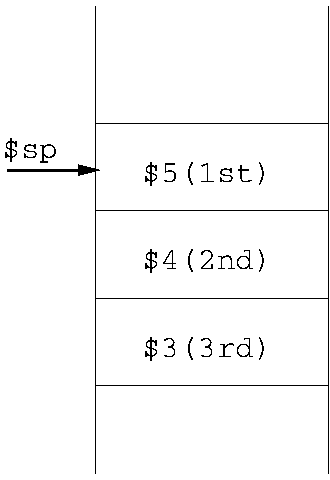
\includegraphics[width=3cm]{stack_fig6_a.eps}
\end{center}
\end{minipage}\\
\hline
\end{tabular}
\\
\textbf{(a) C code}
\hspace{3cm}
\textbf{(b) WRAMP code}
\hspace{3cm}
\textbf{(c) Stack before call}\\

\caption{Passing Parameters to a Function}
\label{fig:parampassing}
\end{footnotesize}
\end{center}
\end{figure}

As you will notice in the previous example, a significant proportion of
the WRAMP code is associated with manipulating the stack pointer. An
alternative and more efficient approach is to calculate the maximum
size that a stack will grow to in a function and pre-allocate this
space as the function is entered. Just before this "parent" function
calls another function it copies the parameters to the appropriate
place in the pre-allocated space. If the function accepts one
parameter, that parameter must be placed at the top of the stack. If a
function accepts two parameters the first parameter must be placed at
the top of the stack and the second placed beneath it. If you think
of the parameters as a list numbered from zero, the position of any
parameter can be calculated as follows:

\begin{center}
$Address = \$sp + ParameterNumber$\\
\end{center}

For example if a function \src{cat(first, second, third)} is going to
be called then first will be placed at \mbox{\src{\$sp} + 0}, second
at \mbox{\src{\$sp} + 1} and third at \mbox{\src{\$sp} + 2}. Figure
\ref{fig:paramcalling}(a) shows an example C code sequence containing two
function calls (one with a single parameter and one with three
parameters) and Figure \ref{fig:paramcalling}(b) shows the WRAMP
assembly code for this sequence.

Once a subroutine has been called it then has to retrieve these
parameters off of the stack so that it can use them. This requires a
number of loads from the current stack. The important part to notice
is that these are not pop operations, as they do not reduce the size
of the stack. The function is simply looking into the stack of the
function that called it to discover the parameters it has been called
with. A function must \textbf{\emph{never}} return with the stack
pointer pointing to a different location than when the function was
called.

A function also needs to be able to return a value to its
parent. Traditional languages only ever allow a function to return a
single value, therefore the use of the stack to return a value is
probably over complex. On the WRAMP architecture, values are returned
to the parent in register 1 (\src{\$1}). Because of this fact,
\src{\$1} is the only exception to the rule that all registers must be
returned with their original contents when a function returns. A
function is actually allowed to change the contents of \src{\$1} even
if it doesn't return any value to its parent. Figure
\ref{fig:paramexample} shows a simple maximum function that is passed
two parameters and returns the larger of the two. As this function is
a leaf function (i.e. calls no other functions) it need not save the
contents of its return address.

%%%%
%
% Figure 7
%
%%%%
\begin{figure}[!hbtp]
\begin{footnotesize}
\begin{center}
\begin{tabular}{|c|c|}
\hline
\begin{minipage}[t]{5cm}
\vspace{\topsep}
\begin{verbatim}

 ...
dog(last);
 ...
cat(first, second, third);
 ...

\end{verbatim}
\end{minipage}
&
\begin{minipage}[t]{8cm}
\vspace{\topsep}
\begin{verbatim}

 # allocate the amount of space on the stack
 # to allow for the call with the largest number
 # or parameters. (in this case 3)
 subui $sp, $sp, 3
  ...

 # The parameter 'last' must be placed on the stack
 # and is currently being stored in $6.
 sw $6, 0($sp)

 # Call the function
 jal dog
  ...

 # Put the parameters for cat onto the stack
 sw $5, 0($sp)    # 'first'
 sw $4, 1($sp)    # 'second'
 sw $3, 2($sp)    # 'third'

 # Call the function
 jal cat
  ...

 # remove the space from the stack.
 addui $sp, $sp, 3

\end{verbatim}
\end{minipage}
\\
\hline
\end{tabular}
\\
\textbf{(a) C code}
\hspace{3.5cm}
\textbf{(b) WRAMP code}
\end{center}
\end{footnotesize}

\caption{Calling multiple functions}
\label{fig:paramcalling}
\end{figure}

\section{Local Variables}
So far we have kept all local variables, such as temporary storage,
loop counters etc. in registers. As there are a small number of
registers it would be a major limit to a language to enforce that it
could have no more local variables than the architecture has
registers. To overcome this limit, the stack is set up so that local
variables can be stored on the stack and only be loaded into registers
temporarily as required. A code segment is shown in Figure
\ref{var_example}(a). Figure \ref{var_example}(b) provides an example
of how the WRAMP code would look if the local variables are kept on the
stack. As you can see, even in this small piece of code there is a
large proportion of the code dealing with fetching and storing the
variables to and from the stack. If you are writing C code it is the
job of a compiler to optimise these areas of the assembly code and
reduce to a minimum the number of these load and store instructions.

\section{The Stack Frame}

All of the discussion so far has been treating the uses of the stack as
separate concepts. In reality all of these are used by C functions to create
a concept called the stack frame. The stack frame is an area on the top of the
stack that has a standard format. Inside this block is space for local
variables, register save and parameter passing for the current function. We
precalculate the size of the stack frame by summing the sizes of each of these
areas. We need space for one item on the stack for every local variable, one
item for each register we save, and one item for each parameter of the function
with the largest number of parameters that we call.

For example if we need to setup a stack frame for a function that needs to
store three local variables and save two registers but calls no other function
we will need a stack frame of size 5.

If we have a non-leaf function that needs 3 local variables, save 4 registers
and the return address, and calls two functions, one of which takes 2 parameter
and the other takes 4 parameters, we will need a stack frame of size 12.

The layout for a complete stack frame is shown in Figure \ref{stackframe}

%%%%
%
% Figure 8
%
%%%%
\begin{figure}[!btp]

\begin{center}
\begin{tabular}{|p{10cm}|}
\hline
\begin{scriptsize}
\begin{verbatim}
parent:
       addi $3, $0, 5
loop:
       beqz $3 endloop
        ...
       jal child
        ...
       subi $3, $3, 1
       j loop

endloop:
       j exit

child:
        ...
       # save register 3 before we overwrite
       # the contents of it
       subui $sp, $sp, 1
       sw $3, 0($sp)

       add $3, $4, $5
        ...
       # restore the old contents of register
       # 3 before we return
       lw $3, 0($sp)
       addui $sp, $sp, 1

       jr $ra
\end{verbatim}
\end{scriptsize}
%$
\\
\hline
\end{tabular}
\end{center}
\

\caption{Example}
\label{fig:paramexample}
\end{figure}

%%%%%%%%%%%%%%%%%%%%%%%%%%%%%%%%

\begin{figure}[!hbtp]
\begin{footnotesize}
\begin{center}
\begin{tabular}{|p{8cm}|}
\hline
\\
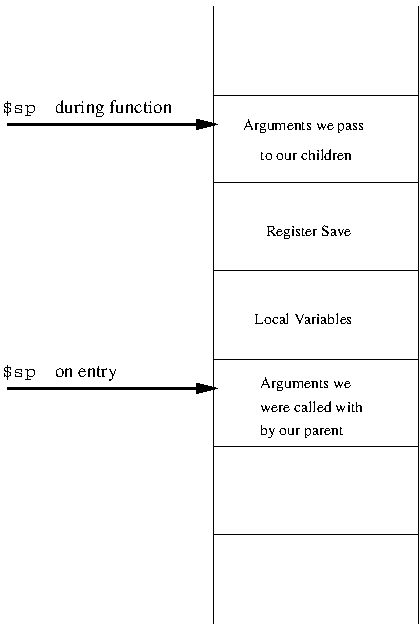
\includegraphics[width=6cm]{stack_fig10.eps}

\\
\hline
\end{tabular}
\end{center}
\end{footnotesize}

\caption{The Stack Frame}
\label{stackframe}
\end{figure}

Figure \ref{stack_example} shows a non-leaf function that calls two
subroutines. The function has zero local variables stored on the
stack, but is a fully compliant function. It sets up a stack frame on
entry and tears it down on exit. It is strongly suggested that you
walk through this code and draw a diagram of the stack frame that this
function creates. Any functions you write that need to be compliant
should contain very similar entry and exit code to this function.

The function is a successive addition multiplication system. It uses a
function called \src{add} to add the two numbers. At the end of the
function it displays the result to the seven segment display using the
\src{writessd} function.

%%%%
%
% Figure 9
%
%%%%
\begin{figure}[!hbtp]
%\begin{footnotesize}
\begin{center}
\begin{tabular}{|c|c|c|}
\hline
\begin{minipage}[t]{5cm}
\begin{scriptsize}
\begin{verbatim}

int i;
int a = 2;
int b = 3;
int result = 0;

for(i = 0; i < a; i++){

   result = result + b;

}

 ...

\end{verbatim}
\end{scriptsize}
\end{minipage}
&
\begin{minipage}[t]{6cm}
\begin{scriptsize}
\begin{verbatim}

func:
       # Allocate space for 4 locals
       subui $sp, $sp, 4

       # Initialise a = 2
       addi $2, $0, 2
       sw $2, 1($sp)

       # Initialise b = 3
       addi $2, $0, 3
       sw $2, 2($sp)

       # Initialise result = 0
       sw $0, 3($sp)

       # Initialise i = 0
       sw $0, 0($sp)

loop:
       # Do the for loop test
       lw $2, 0($sp)  # get i
       lw $3, 1($sp)  # get a
       slt $4, $2, $3
       beqz $4, end

       # perform the loop
       lw $2, 3($sp)  # get result
       lw $3, 2($sp)  # get b
       add $2, $2, $3
       sw $2, 3($sp)  # put result

       # increment i
       lw $2, 0($sp)  # get i
       addi $2, $2, 1
       sw $2, 0($sp)  # put i

       j loop

end:
        ...

\end{verbatim}
\end{scriptsize}
\end{minipage}
&
\begin{minipage}[t]{5cm}
\begin{center}

\vspace{3.5cm}
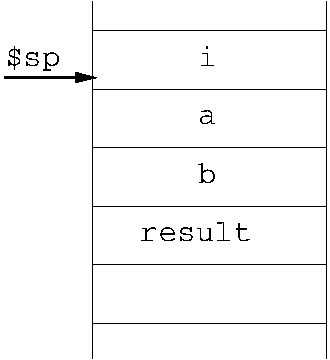
\includegraphics[width=3cm]{stack_fig9_a.eps}

\end{center}
\end{minipage}
\\
\hline
\textbf{(a) C code} & \textbf{(b) WRAMP code} & \textbf{(c) Stack}\\
\hline
\end{tabular}
\end{center}

\caption{Using Variables}
\label{var_example}
\end{figure}

%%%%
%
% Figure 11
%
%%%%
\begin{figure}[!hbtp]
\begin{footnotesize}
\begin{center}
\begin{tabular}{|p{15cm}|}
\hline
\begin{verbatim}

multiply:
        # Setup a stack frame (2 parameters, 5 registers to be saved)
        subui   $sp, $sp, 7
        # Save some registers for us to use
        sw      $6, 2($sp)
        sw      $7, 3($sp)
        sw      $8, 4($sp)
        sw      $9, 5($sp)
        # This is a non-leaf function so we must save the return address
        sw      $ra, 6($sp)

        # Initialise the 'result' variable to zero
        addu    $7, $0, $0
        # Initialise our loop counter
        addu    $6, $0, $0
        # Get our first parameter into $8
        lw      $8, 7($sp)
        # Get our second parameter into $9
        lw      $9, 8($sp)

loop:
        # Use our 1st parameter to control how many times we add our
        # second parameter to itself
        slt     $1, $6, $8
        beqz    $1, exit_loop

        # The first parameter to add is the existing 'result'
        sw      $7, 0($sp)

        # The second parameter we pass is the same as our 2nd parameter
        sw      $9, 1($sp)
        jal     add

        # Save the return value from add back into our 'result' variable
        addu    $7, $0, $1

        # Increment our loop counter
        addui   $6, $6, 1

        j       loop

exit_loop:
        # Write the result to the seven segment display
        sw      $7, 0($sp)
        jal     writessd

        # Return our result to our parent
        addu    $1, $0, $7

        # Restore all the registers we used
        lw      $6, 2($sp)
        lw      $7, 3($sp)
        lw      $8, 4($sp)
        lw      $9, 5($sp)

        # Get our return address back
        lw      $ra, 6($sp)

        # Destroy our stack frame
        addui   $sp, $sp, 7
        # Return
        jr      $ra

\end{verbatim}
%$
\\
\hline
\end{tabular}
\end{center}
\end{footnotesize}

\caption{Example}
\label{stack_example}
\end{figure}

\chapter{REX I/O Devices}
\label{chapter:io}
\section{Introduction}

The Basys board provides a number of I/O devices. This document
describes the devices and the way in which WRAMP code can interact
with them. There are three major I/O devices: a dual serial port, a
parallel port and a programmable timer.

All Basys I/O devices are memory mapped. This means that to access a
device, WRAMP code simply reads or writes to special memory locations
using the standard load word (\src{lw}), and store word
(\src{sw}) instructions.

The base memory addresses of all of the devices are provided in
Table~\ref{table:base_addr}. The details of how to use each of the
devices forms the body of this document.

\begin{table}[h]
\begin{center}
\begin{tabular}{|l|l|}
\hline
\textbf{Device} & \textbf{Base Address} \\
\hline
First Serial Port & \LOCFSPBASE \\
\hline
Second Serial Port & \LOCSSPBASE \\
\hline
Timer Base & \LOCTIMEBASE \\
\hline
Parallel Port & \LOCPARABASE \\
\hline
\end{tabular}
\caption{I/O Device Base Addresses}
\label{table:base_addr}
\end{center}
\end{table}

\section{Serial Devices}

The Basys board provides two independent RS232 serial interfaces.

Each of these ports can be attached to the same computer, using two
Micro-USB cables. A Linux computer can interface with these ports
with either \filename{remote} or any other terminal emulator that can
communicate with serial devices. They will usually appear somewhere
similar to \src{/dev/ttyUSB1}.

The first serial port is attached to the Linux machine from the
micro-USB on the top left of the board. This port is used by the
monitor software on the Basys board to communicate with the user and 
to allow software to be uploaded to the Basys board. The second serial
port is attached to the Linux machine via the Pmod peripheral micro-USB.

The programmer's view of a serial interface consists of five registers.
The names of these registers and their addresses, expressed as offsets
from the base address, are provided in
Table~\ref{table:serial_offsets}. The base address for the first
serial port is \src{\LOCFSPBASE} and the base address for the
second serial port is \src{\LOCSSPBASE}.

\begin{table}[h]
\begin{center}
\begin{tabular}{|l|c|}
\hline
\textbf{Register name} & \textbf{Offset} \\
\hline
Serial Transmit Data Register & 0 \\
\hline
Serial Receive Data Register & 1 \\
\hline
Serial Control Register & 2 \\
\hline
Serial Status Register & 3 \\
\hline
Serial Interrupt Acknowledge Register & 4 \\
\hline
\end{tabular}
\caption{Serial Port Register Offsets}
\label{table:serial_offsets}
\end{center}
\end{table}

The serial ports provided on the Basys board can operate in either
polled or interrupt driven I/O modes. Interrupt I/O is be disabled
by default.

\subsection{Serial Transmit Data Register}

The Transmit Data Register (TDR) is a write-only register. A character
will be transmitted by writing the value into this register. The
serial port status register indicates if a value is permitted to be
written to this register. If a character is written to this register
without first checking the status register, it is be possible to lose
characters. If transmit data sent interrupts are enabled, an interrupt
will be triggered when this register becomes empty indicating that
another character can now be sent. Some example WRAMP code to transmit
a single character is given in Figure~\ref{code:serial_tran}.

\begin{figure}[h]
\begin{footnotesize}
\begin{center}
\begin{tabular}{|p{8cm}|}
\hline
\begin{verbatim}
            . . .
           # Put the character we want to send in $9
           addi $9, $0, 'A'
           
     check: 
           # Get the first serial port status
           lw   $11, 0x70003($0)
           # Check if the TDS bit is set
           andi $11, $11, 0x2
           # If not, loop and try again
           beqz $11, check
           # Serial port is now ready so
           # transmit character
           sw   $9,  0x70000($0)
            . . .
\end{verbatim}
\\
\hline
\end{tabular}
\end{center}
\end{footnotesize}
\caption{Simple Transmit Code}
\label{code:serial_tran}
\end{figure}

\subsection{Serial Receive Data Register}

The Receive Data Register (RDR) is a read-only register. When a
character is received from the serial line, it appears in this
register. When a character arrives the status register will reflect
this change. If receive data ready interrupts are enabled, an
interrupt will be triggered when data arrives in this register. An
example of a simple polled receive routine is shown in
Figure~\ref{code:serial_rec}.

\begin{figure}[h]
\begin{footnotesize}
\begin{center}
\begin{tabular}{|p{8cm}|}
\hline
\begin{verbatim}
            . . .
     check: 
           # Get the first serial port status
           lw   $11, 0x70003($0)
           # Check if the RDR bit is set
           andi $11, $11, 0x1
           # If not, loop and try again
           beqz $11, check
           # Serial port now has a character.
           # Get it into $9
           lw   $9,  0x70001($0)
            . . .
\end{verbatim}
\\
\hline
\end{tabular}
\end{center}
\end{footnotesize}
\caption{Simple Receive Code}
\label{code:serial_rec}
\end{figure}

\newpage
\subsection{Serial Control Register}

This register allows line parameters such as serial bit rate to be
set. The serial ports are configured appropriately by the monitor for
the setup distributed with \filename{remote} by default. Unless you know
that you specifically need to change something in this register you
should leave it as default. Keep in mind that the second serial port
is configured at 38400 baud, so any terminal emulators used to interact
with it should be set as such.

The control register also controls when the serial port will cause an
interrupt. The serial port can selectively cause an interrupt when a
character is received into the receive data register, the transmit
data register becomes empty or on an error condition. Any combination of
these can be enabled or disabled at one time. To enable interrupts to
be used by the serial port under specific circumstances a `\src{1}'
should be written to the appropriate location. If an interrupt has
occurred it must be acknowledged by writing into the serial interrupt
acknowledge register.

The \WRAMPmon\ will initialise the serial port so that no
interrupts are enabled.

The control register is a read/write register. Writes to this register
have an immediate effect on the line settings.

\begin{figure}[h]
\begin{center}
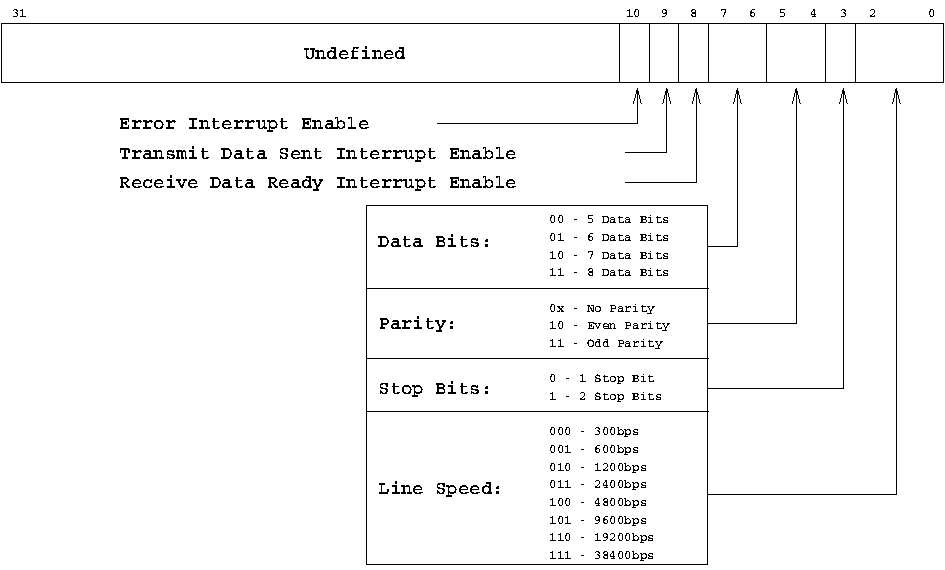
\includegraphics[width=0.8\textwidth]{serial_cr.pdf}
\caption{The Serial Control Register}
\label{serial_cr_pic}
\end{center}
\end{figure}

\noindent
eg. To configure a serial interface to operate with no interrupts
enabled, at 9600 bits per second, with 8 data bits, no parity and 1
stop bit, the value `\src{00011000101}' would be written to the
control register.

\subsection{Serial Status Register}

The status register is a read-only register, which gives error and
status information about the serial interface. It allows the
programmer to see if data has been received, sent, or if an error
condition is present.

The Transmit Data Sent (TDS) bit will be set to `\src{1}' as soon
as the transmit data register is empty. Checking that this bit is set
allows WRAMP code to ensure that it will not overwrite any data by
placing another character into the transmit data register. This bit
will automatically be cleared if the transmit data register becomes
full.

Similarly, the Receive Data Ready bit will be set to `\src{1}' as soon
as there is new valid data in the receive data register. A read from
the receive data register automatically clears this bit.

\begin{figure}[h]
\begin{center}
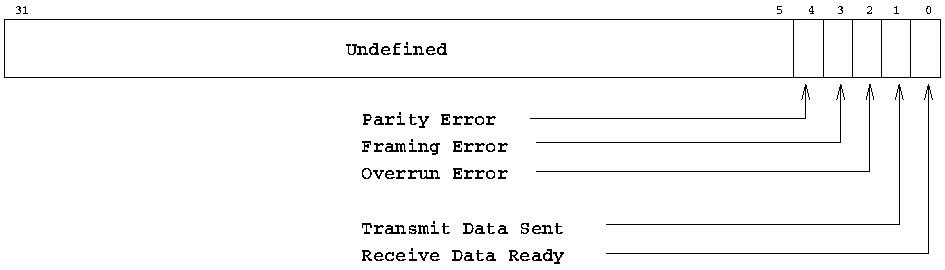
\includegraphics[width=0.8\textwidth]{serial_sr.pdf}
\caption{The Serial Status Register}
\label{serial_sr_pic}
\end{center}
\end{figure}

\noindent
eg. If the value `\src{00001}' was read from the status register
then we could determine that a character has been received without
error, and is available in the receive data register.

\subsection{Serial Interrupt Acknowledge Register}

The interrupt acknowledge register is a read/write register. When the
serial interface has generated an interrupt this register allows the
program to determine the reason for the interrupt as well as
acknowledge interrupts that have been dealt with.

To acknowledge an interrupt a zero (`\src{0}') should be written
over the current status field for the type of interrupt being
acknowledged. Most often it will be the desire of the programmer to
acknowledge all of the possible serial port interrupts in one
instruction. This can be achieved by storing register \reg{0} to
the interrupt acknowledge register.

\begin{figure}[h]
\begin{center}
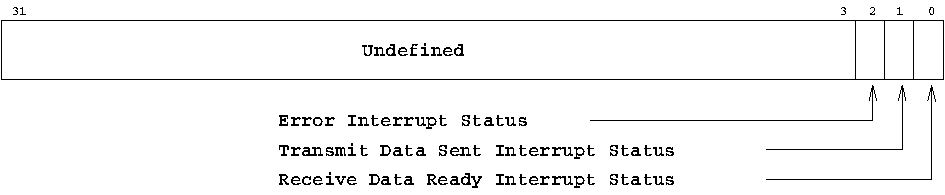
\includegraphics[width=0.8\textwidth]{serial_iack.pdf}
\caption{The Serial Interrupt Acknowledge Register}
\label{serial_iack_pic}
\end{center}
\end{figure}

\noindent
eg. If the value `\src{010}' was read from the interrupt
acknowledge register we could determine that the cause of the
interrupt was the transmit data register becoming empty. If the value
`\src{000}' was written to the interrupt acknowledge register all
outstanding serial port interrupts would be acknowledged.

\section{Parallel Interface}

The parallel interface on the Basys board provides an input interface
from a bank of 16 on-off switches and three momentary push-buttons, as
well as an output interface to four LED Seven Segment Displays (SSDs)
and 16 LEDs.
Parallel interrupts, if enabled, will be generated on any switch or
push-button state change.

The programmer's view of the parallel interface consists of 10
registers. The names of these registers and their addresses,
expressed as offsets from the base address, are provided in
Table~\ref{table:parallel_offsets}. The base address for the parallel
port is \src{\LOCPARABASE}. Please note that due to the inclusion of
two more SSDs in the Basys implementation, the original two SSDs can
be addressed from two locations to allow for both backwards compatibility
and to have all 4 SSDs in sequential addresses.

\begin{table}[h]
\begin{center}
\begin{tabular}{|l|c|}
\hline
\textbf{Register name} & \textbf{Offset} \\
\hline
Parallel Switch Register & 0 \\
\hline
Parallel Push Button Register & 1 \\
\hline
Parallel Lower Left SSD Register & 2 \\
\hline
Parallel Lower Right SSD Register & 3 \\
\hline
Parallel Control Register & 4 \\
\hline
Parallel Interrupt Acknowledge Register & 5 \\
\hline
Parallel Upper Left SSD Register & 6 \\
\hline
Parallel Upper Right SSD Register & 7 \\
\hline
Parallel Lower Left SSD Register & 8 \\
\hline
Parallel Lower Right SSD Register & 9 \\
\hline
Parallel LED Register & 10 \\
\hline
\end{tabular}
\caption{Parallel Port Register Offsets}
\label{table:parallel_offsets}
\end{center}
\end{table}

\subsection{Parallel Switch Register}

The switch register is a read-only register. A read from this register
returns a bit pattern with bits set corresponding to the switches that
are on.

\begin{figure}[h]
\begin{center}
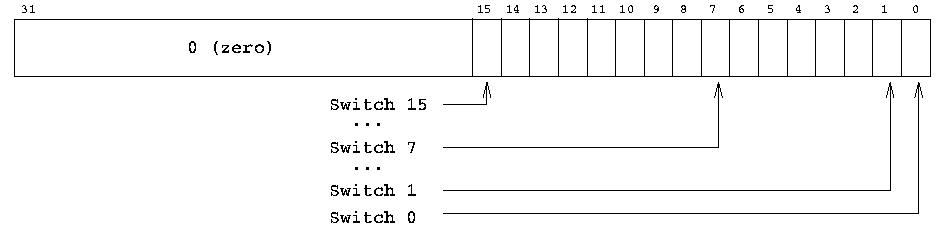
\includegraphics[width=0.8\textwidth]{switch_reg.pdf}
\caption{The Switch Register}
\label{switch_reg_pic}
\end{center}
\end{figure}


\subsection{Parallel Push Button Register}

The push button register is a read-only register. A read from this
register returns a bit pattern in the low order 3 bits corresponding
to the push buttons that are currently being depressed.

\begin{figure}[h]
\begin{center}
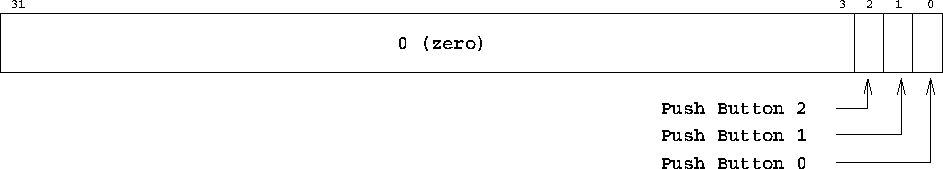
\includegraphics[width=0.8\textwidth]{button_reg.pdf}
\caption{The Push Button Register}
\label{button_reg_pic}
\end{center}
\end{figure}

\subsection{Parallel Left, Right, Upper and Lower SSD Registers}

The four SSD Registers are read/write registers. These
registers contain the value to be displayed on their respective Seven
Segment Display. 

If the hexadecimal to seven-segment decode bit is enabled in the
parallel control register, four bits of input will be decoded into a
single hexadecimal digit and displayed on the seven-segment display.

If the hexadecimal to seven-segment decode bit is turned off, then
each segment can be individually controlled by a single bit of the
input. The displays are made up of seven segments and a decimal point.
The first eight bits of input turn on the segments as shown in
Figure~\ref{fig:ssd}.
Hex-decode is enabled by default.

In this manual, the terms Upper and Lower refer to the left and right
pairs of SSDs respectively. As such, the far left SSD is the Upper Left
SSD (addressed with offset 6), and the second from the left is the Lower
Left SSD (addressed with either offset 8 or 2).

\begin{figure}[h]
\begin{center}
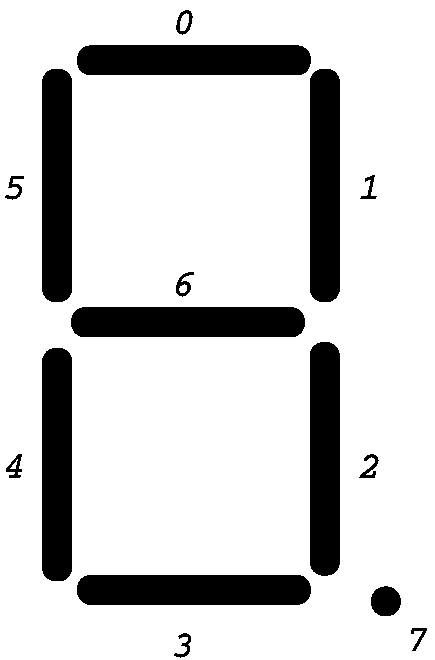
\includegraphics[width=0.12\textwidth]{ssd.pdf}
\caption{Seven-segment display bit encoding}
\label{fig:ssd}
\end{center}
\end{figure}

\subsection{Parallel Control Register}

The Parallel Control Register is a read/write register, which allows
for control over the parallel interface.

\begin{figure}[h]
\begin{center}
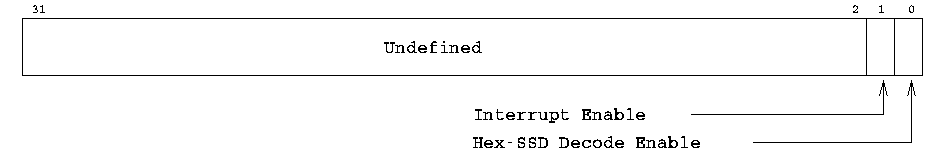
\includegraphics[width=0.8\textwidth]{parallel_cr.pdf}
\caption{The Parallel Control Register}
\label{parallel_cr_pic}
\end{center}
\end{figure}

eg. To enable interrupts on switch changes and force hex-SSD decoding
on the displays, a value of `\src{11}' would be written to
the parallel control register.

\subsection{Parallel Interrupt Acknowledge Register}

The Interrupt Acknowledge Register is a read/write register. This
register allows a program to determine the parallel port interrupt
status as well as acknowledge interrupts that have been dealt with.

\begin{figure}[h]
\begin{center}
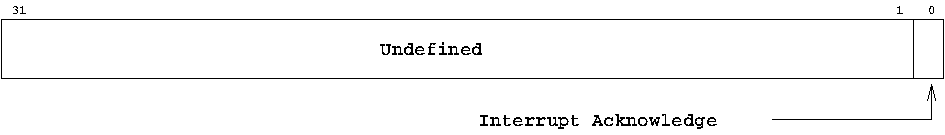
\includegraphics[width=0.8\textwidth]{parallel_iack.pdf}
\caption{The Parallel Interrupt Acknowledge Register}
\label{parallel_iack_pic}
\end{center}
\end{figure}

eg. To acknowledge an outstanding parallel port interrupt `\src{0}'
would be written to the parallel interrupt acknowledge register.

\subsection{LED Register}

The LED register is a read/write register. This
register allows a program to selectively illuminate the bank of 16 LEDs
sitting above the switches.

\begin{figure}[h]
\begin{center}
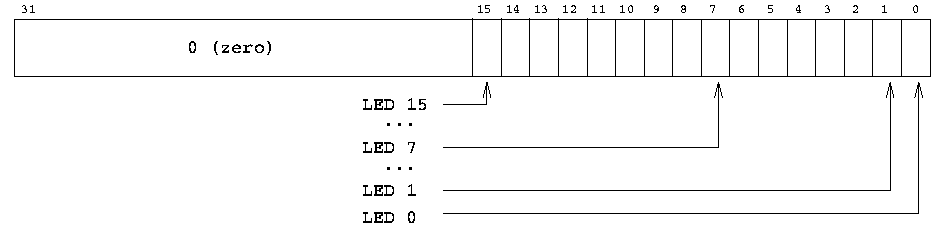
\includegraphics[width=0.8\textwidth]{led_reg.pdf}
\caption{The LED Register}
\label{LED_pic}
\end{center}
\end{figure}

\section{Programmable Timer}

The Programmable Timer on the Basys board allows for the generation of
interrupts at time intervals from about 1ms to 30s, with a resolution
of around 0.5ms.

The timer has an internal 16-bit register. This register is decremented
at a constant rate of 2400Hz. Once this register reaches
\src{0x0000} an interrupt is triggered. The starting value for the
timer is controlled by altering the value in the timer load register.

Please note due to the new hardware, a rate of exactly 2400Hz was not attainable.
Instead of picking another whole number, the clock rate was approximated
to maintain backwards compatibility. Internally, a register counts down from 1302 
at a rate of 6.25MHz, then inverts a clock signal to the timer.
Every second inversion of this signal will decrement the timer's counter.
This yields an approximate ((6.25Mhz/1302)/2) = 2400.153609831Hz.
This has an error of approximately 5 seconds per 24 hours of timer operation.

The timer can be configured to automatically reload the starting count
value and continue counting immediately after it expires.

The programmer's view of the timer consists of four registers.  The
names of these registers and their addresses, expressed as offsets
from the base address, are provided in
Table~\ref{table:timer_offsets}.  The base address for the timer is
\src{\LOCTIMEBASE}.

\begin{table}[h]
\begin{center}
\begin{tabular}{|l|c|}
\hline
\textbf{Register name} & \textbf{Offset} \\
\hline
Timer Control Register & 0 \\
\hline
Timer Load Register & 1 \\
\hline
Timer Count Register & 2 \\
\hline
Timer Interrupt Acknowledge Register & 3 \\
\hline
\end{tabular}
\caption{Timer Register Offsets}
\label{table:timer_offsets}
\end{center}
\end{table}

\subsection{Timer Control Register}

The Timer Control Register is a read/write register, that allows the
user to enable and control aspects of the timer operation. The timer
has two primary modes of operation, automatic restart and single-shot
mode. If the timer is set to automatic restart, as soon as the timer
expires, an interrupt is triggered and the timer immediately starts
counting down again. In single-shot mode the timer will copy the value
from the timer load register only once when the timer is enabled and
will count down to zero. Once the timer reaches zero an interrupt will
be triggered and the timer will be disabled.

\begin{figure}[h]
\begin{center}
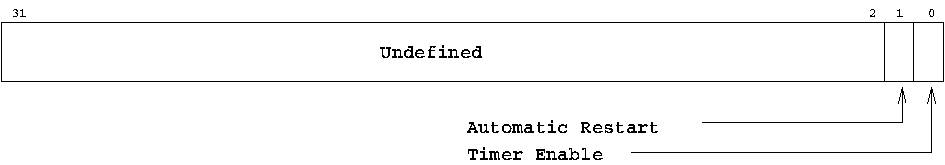
\includegraphics[width=0.8\textwidth]{timer_cr.pdf}
\caption{The Timer Control Register}
\label{timer_cr_pic}
\end{center}
\end{figure}

\subsection{Timer Load Register}

The Timer Load Register is a read/write register. This register allows
the user to specify the starting count value. The starting count value
is a 16-bit value with the upper 16 bits being ignored.

\subsection{Timer Count Register}

The Timer Count Register is a read-only register. Reading from this
register returns the current value in the 16-bit internal count
register.

\subsection{Timer Interrupt Acknowledge Register}

The Interrupt Acknowledge Register is a read/write register. This
register allows a program to detect a timer overrun as well as
acknowledge interrupts that have been dealt with.

The overrun detected bit will be set if the timer is set to automatic
restart and the timer expired again before the previous interrupt was
acknowledged. This allows a program to detect if it is unable to
service the timer interrupt fast enough.

The overrun bit must be manually reset by writing a `\src{0}' to
it's location.

\begin{figure}[h]
\begin{center}
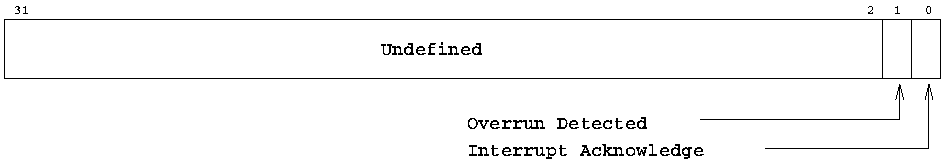
\includegraphics[width=0.8\textwidth]{timer_iack.pdf}
\caption{The Timer Interrupt Acknowledge Register}
\label{timer_iack_pic}
\end{center}
\end{figure}

eg. If the value `\src{11}' was read from the interrupt acknowledge
register we could determine that the timer has overrun since we last
acknowledged an interrupt. If `\src{00}' was written to the timer
interrupt acknowledge register we will acknowledge any outstanding
interrupts and ensure the overrun bit is reset to zero.

\subsection{Timer Example}

To configure the timer to interrupt at a specific period the first
step is to calculate the timer load value. This value can be
calculated simply by multiplying the timer frequency by the required
time between interrupts. For example, if we want the timer to generate
an interrupt once every ten seconds we would calculate it as follows:

\begin{center}
Timer Load = 2400Hz * 10s = 24000 = 0x5dc0
\end{center}

Some simple code to initialise the timer to automatically restart and
interrupt once every ten seconds is given in
Figure~\ref{code:timer_init}.

\begin{figure}[h]
\begin{footnotesize}
\begin{center}
\begin{tabular}{|p{8cm}|}
\hline
\begin{verbatim}
            . . .
           # Make sure there are no old interrupts
           # still hanging around
           sw   $0, 0x72003($0)
           # Put our auto load value in
           addi $11, $0, 0x5dc0
           sw   $11, 0x72001($0)
           # Enable the timer and autorestart
           addi $11, $0, 0x3
           sw   $11, 0x72000($0)
            . . .
\end{verbatim}
\\
\hline
\end{tabular}
\end{center}
\end{footnotesize}
\caption{Simple Timer Initialisation}
\label{code:timer_init}
\end{figure}

\chapter{Exceptions}
\label{chapter:exceptions}
\section{Introduction}

Modern processors can execute millions of instructions each
second. This means that when a processor is polling an I/O device for
data or status information which may only change very infrequently, it
is wasting a lot of time where it could be doing some worthwhile
processing.  It would be more efficient for a device to signal the CPU
when something happens (eg. a character is received at the serial
port, the user flicks a switch, or a certain time has elapsed).

Also consider what should happen if something goes wrong when a
program is executing. What should happen if an attempt is made to
divide by zero? What should happen if you add two numbers and the
result will not fit in 32 bits?

This is why almost all modern processors provide support for
exceptions. Exceptions provide a mechanism which allows the processor
to be executing code, and when a certain condition occurs, to deal
with that condition, and then return to what it was doing initially.

The terms `exception' and `interrupt' are often used
interchangeably. There are varying opinions on the exact definitions of
these terms, however the term `interrupt' generally refers only to the
exceptions which are caused by something outside the processor
(eg. the serial port, or the timer).

The WRAMP processor allows for four internal exceptions. These are:

\begin{itemize}
\item Arithmetic Exception (ie. Divide-by-zero, or Overflow)
\item Breakpoint Exception (a 'break' instruction has been executed)
\item System Call Exception (a 'syscall' instruction has been
executed)
\item General Protection Fault Exception (eg. an illegal instruction
is encountered)
\end{itemize}

WRAMP provides eight external interrupts. The external interrupts are 
simply wires coming into the processor, and so can be connected to any 
devices.  These are called IRQ0 (for Interrupt ReQuest) to IRQ7. On the 
REX board these are connected as follows:

\begin{center}
\begin{tabular}{|c|l|c|l|}
\hline
\textbf{IRQ \#} & \textbf{Description} & \textbf{IRQ \#} &
\textbf{Description} \\
\hline
0 & Unconnected & 4 & Serial Port 1 Interrupt \\
\hline
1 & User Interrupt Button & 5 & Serial Port 2 Interrupt\\
\hline
2 & Timer Interrupt & 6 & Unconnected \\
\hline
3 & Parallel Interrupt &7 & Unconnected \\
\hline
\end{tabular}
\end{center}

Exceptions can be thought of as similar to subroutine calls. The
processor is executing a block of code, when an exception occurs,
causing the processor to jump to a location called the `exception
vector'.  The processor then executes the code at this location (known
as the `exception handler' or `exception routine'), and returns to the
point at which it was executing when the exception occurred.

For this mechanism to work, we will need registers to store things
like the exception vector (the address of the exception handler), and
the address of the instruction to return to after the exception has
been handled. The general purpose registers are not suitable for this,
because a program may be using them, and if an exception occurs, then
there may be unpredictable results. For this reason the WRAMP
processor provides a special set of registers that are used for
advanced processor features like exceptions.

Like the general purpose registers (\reg{0} - \reg{ra}), there are 16 special
purpose registers. Because each has a specific use, they are called by
their names rather than their numbers. The special registers concerned
with exceptions are:

\begin{itemize}
\item \reg{cctrl} - CPU Control Register
\item \reg{estat} - Exception Status Register
\item \reg{evec} - Exception Vector Register
\item \reg{ear} - Exception Address Register
\item \reg{ers} - Exception Register Save
\end{itemize}

All special purpose registers cannot be operated on directly like
the general purpose registers. Rather, two instructions are provided
to allow register contents to be copied from a general purpose
register to a special purpose register, or vice-versa. These
instructions are \src{movsg} (move special register to general
register), and \src{movgs} (move general register to special
register). Details on these instructions can be found in the WRAMP
instruction reference in Appendix \ref{appendix:instr}.

The next sections will describe the format of each of these special
purpose registers. Contained in these descriptions will often be
introductions to new concepts and ideas. As such this chapter is best
read once end-to-end to ensure that all concepts are introduced fully.

\section{CPU Exception Control Registers}

\subsection{\$cctrl - CPU Control Register}

\begin{figure}[h]
\begin{center}
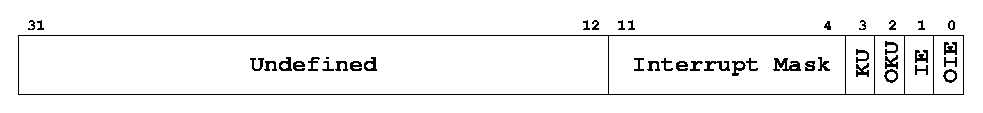
\includegraphics[width=\textwidth]{cctrl.eps}
\caption{\$cctrl - CPU Control Register}
\label{cctrl_pic}
\end{center}
\end{figure}

The CPU control register controls almost all of the functionality
related to the WRAMP exception mechanism. There are three main
sections of this register:

\begin{itemize}
\item Interrupt Enable (IE)
\item Kernel/User Mode (KU)
\item Interrupt Mask
\end{itemize}

\subsubsection{Interrupt Enable}

This flag provides a global interrupt enable. If this location is set
to `\src{0}' then no interrupts can be triggered. This flag
\emph{only} affects external interrupts. There is no way on the WRAMP
processor to disable internal exceptions.

Interrupts that occur while the global interrupt enable is turned off
will be held back. As soon as interrupts are again enabled by writing
a `\src{1}' into this location the interrupt mask will be consulted
to discover if that specific interrupt is enabled. See
Section~\ref{sec:imask} for more information about the interrupt mask.

The CPU will automatically set the IE bit to `\src{0}' whenever an
exception of any type occurs. This prevents the exception handler
from being interrupted by another interrupt.

\subsubsection{Interrupt Mask}
\label{sec:imask}

This provides a way to selectively turn on and off individual external
interrupts. This field has a bit corresponding to each of the eight
possible external interrupts (IRQ0 - IRQ7). Bit 4 of the CPU control
register corresponds to IRQ0, bit 5 to IRQ1 and so on.

The interrupt mask field is only consulted if the global interrupt
enable (IE) flag is set. If an interrupt occurs and the global
interrupt flag is set but the individual interrupt mask is disabled
then the interrupt will be held back. As soon as both the global
interrupt enable and the specific interrupt mask bits are set then the
interrupt will occur.

\subsubsection{Kernel User Mode}

The WRAMP CPU has two modes of operation, kernel and user mode. If
there is a `\src{1}' in the KU bit the CPU is in kernel mode. If
the KU bit is set to `\src{0}' then the CPU is in user mode. 

If the CPU is running in kernel mode it will execute all instructions and
allow access to all areas of memory. If the CPU is running in user
mode programs are not allowed to use any of the three instructions
which deal with the special register file (\src{movsg, movgs, rfe})
and may not be able to access all memory locations. If a program
running in user mode attempts to use one of these instructions, or to
access protected memory the CPU will cause a General Protection Fault
exception. %TODO see section on the MPU

The CPU will automatically set the KU bit to `\src{1}' whenever an
exception of any type occurs. This allows the exception handler to
operate in kernel mode, allowing it full access to all instructions
and memory locations.

\subsection{\$estat - Exception Status Register}

\begin{figure}[h]
\begin{center}
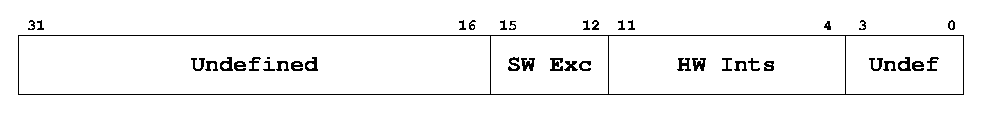
\includegraphics[width=\textwidth]{estat.eps}
\caption{\$estat - Exception Status Register}
\label{estat_pic}
\end{center}
\end{figure}

The exception status register provides the exception handler with the
ability to discover which exceptions caused it to be invoked. The
exception status register has a single bit flag for each external IRQ
line. Bit 4 of the status register corresponds to IRQ0, bit 5 to IRQ 1
and so on. These locations are exactly the same as the locations of
the interrupt mask fields in the CPU control register as described in
Section~\ref{sec:imask}. In addition to the eight external interrupt
sources the status register also provides the status for the four CPU
internal exception sources. 

The full list of all exception sources and their related status
register bit is given in Table~\ref{table:sta_loc}.

Most exception handlers will wish to check which exception caused them
to be called. Provided in Figure~\ref{code:stat_check} is code that
checks if a specific interrupt caused the handler to be called. If any
other interrupt or exception is currently high then the code will call
an old handler to deal with the exception. The code to save the
address of an old handler is given in Figure~\ref{code:evec} and
discussed in Section~\ref{sec:evec}.

\begin{table}[h]
\begin{center}
\begin{tabular}{|l|c|}
\hline
\textbf{Exception source} & \textbf{Bit location} \\
\hline
IRQ0 & 4 \\
\hline
IRQ1 - User Interrupt Button & 5 \\
\hline
IRQ2 - Timer Interrupt & 6 \\
\hline
IRQ3 - Parallel Interrupt & 7 \\
\hline
IRQ4 - Serial Port 1 Interrupt & 8 \\
\hline
IRQ5 - Serial Port 2 Interrupt & 9 \\
\hline
IRQ6 & 10 \\
\hline
IRQ7 & 11 \\
\hline
General Protection Fault Exception & 12 \\
\hline
System Call Exception & 13 \\
\hline
Breakpoint Exception & 14 \\
\hline
Arithmetic Exception & 15 \\
\hline
\end{tabular}
\caption{Exception Status Register Fields}
\label{table:sta_loc}
\end{center}
\end{table}

\begin{figure}[h]
\begin{footnotesize}
\begin{center}
\begin{tabular}{|p{10cm}|}
\hline
\begin{verbatim}
          . . .
  handler:

        # Get the status register
        movsg   $13, $estat

        # Inspect only the bits we are interested in. We want 
        # to check that no bits from the sw exceptions or 
        # hardware exceptions, other than the one we were 
        # expecting, are enabled.
        #
        # This code is looking for an IRQ4 interrupt.
        andi    $13, $13, 0xfef0
         
        # If the result of this is zero then no other 
        # exceptions are enabled so it must be our interrupt
        # that caused us to be called.
        beqz    $13, handle_interrupt 

        # Otherwise there was another exception that has 
        # occurred, so call the old handler
        lw      $13, old_vector($0)
        jr      $13

  handle_interrupt:

        # This is where we deal with the interrupt.
           . . .
\end{verbatim}
\\
\hline
\end{tabular}
\end{center}
\end{footnotesize}
\caption{Checking the Status Register}
\label{code:stat_check}
\end{figure}

\subsection{\$evec - Exception Vector Register}
\label{sec:evec}

When an exception occurs the CPU needs to jump to the exception
handler. The CPU must therefore know what address the exception
handler starts at.

The address of the exception handler is stored in the exception vector
register. The CPU jumps to this location whenever an exception occurs.

If a program is replacing an existing exception handler, but will still
need to call the old handler for certain exceptions, the code must
be careful to save the address of the old exception handler. This
allows the new handler to decide if it will deal with this exception,
and if not, call the old handler.

A section of WRAMP code to save the address of an old exception
handler, load the address of the new handler and save this to the
exception vector is given in Figure~\ref{code:evec}.

\begin{figure}[h]
\begin{footnotesize}
\begin{center}
\begin{tabular}{|p{8cm}|}
\hline
\begin{verbatim}
          . . . 
        # Get the old exception vector
        movsg   $4, $evec
        # And save it
        sw      $4, old_vector($0)

        # Get the address of our handler
        la      $4, handler
        # And put it in the exception vector register
        movgs   $evec, $4

            . . .
	
   handler:
        # The exception handler goes here

            . . .

   old_vector:
        .word   0

\end{verbatim}
%$
\\
\hline
\end{tabular}
\end{center}
\end{footnotesize}
\caption{Saving and Initialising the Exception Vector}
\label{code:evec}
\end{figure}

\subsection{\$ear - Exception Address Register}

An exception routine must be able to return to the point in program code at
which the exception occurred.  To allow this, when an exception occurs the
WRAMP pocessor automatically saves the address of the next instruction
that would have been executed into \reg{ear} - the Exception Address
Register.

When the exception routine has completed its processing, it executes a
Return From Exception, or \src{rfe} instruction. Amongst other things, this
instruction causes a jump to the address contained in \reg{ear}.

In some circumstances an exception routine may wish to know the address at
which the exception was invoked, or may wish to alter the address to which
the \src{rfe} will return. This can be achieved by inspecting and/or modifying
the contents of the \reg{ear}.

\subsection{\$ers - Exception Save Register}

It is vital that an exception routine does not change the contents of the
general purpose registers when it returns to the main program, as changes
may cause the main program to behave in an unpredictable fashion.

However, for the exception handler to determine the cause of the exception,
it requires a general purpose register into which it can copy
\reg{estat}. The WRAMP processor makes general purpose register \reg{13}
available for this by automatically copying it to the Exception Save
Register (\reg{ers}) when an exception occurs. The opposite of this happens
when an \src{rfe} instruction is executed - \reg{ers} is copied into
\reg{13}.

This means that exception handler code must only change \reg{13}.  If
it needs other registers it must save their contents before using
them.  They must then be restored before returning to the main
program.

\section{User Interrupt Button}

The REX board provides a simple method for creating an
interrupt. There is a button located on the front of the case, next to
the reset button labeled ``INTR''. When this button is pressed IRQ1,
the ``User Interrupt Button'', interrupt will be triggered. If this
interrupt is unmasked and the global interrupt enable is turned on in
\src{\$cctrl} an exception will occur.

This button provides a simple way to test an exception handler as it
avoids problems that could be caused by mis-configuration of the I/O
device that is being used to provide the exception.

Like all other REX interrupt sources the user interrupt button needs
to be acknowledged each time an exception occurs. To acknowledge a
``User Interrupt'' you store zero to the address
\src{0x7f000}. Unlike the other I/O devices on the REX board you do
not need to enable or disable the user interrupt button. If IRQ1 is
unmasked in \src{\$cctrl} and interrupts are enabled the button
will cause an exception when pressed.

\section{Using Exceptions}

Writing a program that uses exceptions is best done as a step by step
process. If you attempt to write an entire program that uses exceptions
from start to finish in one hit, then there is a good chance you will never
debug any problems that may arise.

The first thing that you will need when writing your first handler is a
simple program that will run as the main loop of your code. You use this to
ensure that the exception routine is returning to your original code
correctly. A program which reads the value on the switches and writes this
to the seven segment display is ideal. Obviously you should do this in a
polled fashion.

Next you should write a very simple piece of code that will constitute
your exception handler. A suggested program is one which writes a
single character to a serial port. As this code will eventually be run
from inside your exception handler it must transmit this character
using polled I/O.

Test that both of these pieces of code work in a normal environment with no
exceptions. Also ensure that the code which will act as your exception
handler makes use only of \reg{13}.

The next step is to actually enable an interrupt and get the handler
you just wrote to be run. As suggested above the best source for your
first interrupt is the user interrupt button, IRQ1. The things that
you need to do to get this working are:

\begin{itemize}
\item Save the old exception handler address
\item Put the address of your new handler into \src{\$evec}
\item Make sure that there are no old interrupts hanging around by
storing \src{\$0} to the acknowledge register of the device you
will be using. For IRQ1 the acknowledge register is at address
\src{0x7f000}.
\item Configure the CPU control register to enable interrupts. This
takes a number of smaller steps:
\begin{itemize}
\item Get the current value of \src{\$cctrl}
\item Disable all interrupts.
\item Enable the interrupt you wish to use (IRQ1) and set the global
interrupt enable to `\src{1}'. Be careful that you do not alter any
other locations in this register besides the ones specified.
\item Store this value back into \src{\$cctrl}.
\end{itemize}
\end{itemize}


You will need to add some code to the simple exception handler that
you just wrote to make it a complete exception handler. Your exception
handler must start with code to detect if the interrupt is one that
you wish to deal with. Some example code for this is given in
Figure~\ref{code:stat_check}. Beware that you will need to alter this
code so that it checks for the correct interrupt. If you are using the
user interrupt button you should make sure the code checks that only
IRQ1 is high.

Next you must remember to acknowledge the interrupt. If you do not
acknowledge the interrupt then as soon as your exception routine exits
it will be instantly called again. This means you code will be stuck
in an infinite loop, probably printing character after character to
the serial port.

The very final instruction of you exception handler must be an
\src{rfe}. Only use an \src{rfe} instruction in code that you
are sure will only be called as part of an exception handler. If you
use the \src{rfe} instruction when you are not inside an exception
handler you may find your code will get stuck in an infinite loop or
crash.

If this code is now working, then you should have a character appearing
each time you push the user interrupt button as well as the value on the
switches constantly being displayed on the seven segment display. If so,
try altering your code so that you use one of the other I/O devices to
cause exceptions.

\section{Exception Procedure}

What actually happens when an exception occurs? The CPU performs a
number of operations when an exception occurs but they are all pretty
simple. The CPU does the following:

\begin{itemize}
\item Copy the IE bit into the OIE bit
\item Set IE to zero
\item Copy the KU bit into the OKU bit
\item Set KU to one
\item Set the \reg{estat} register to reflect the cause of the exception
\item Copy \reg{13} into \reg{ers}
\item Save the program counter into \reg{ear}
\item Set the program counter to the contents of \reg{evec}
\end{itemize}

At this point the next instruction is fetched. This instruction is the
first instruction of the exception handler and therefore the handler
is now running.

Once the exception handler has finished the final instruction it will
call will be an \src{rfe}. The CPU takes the following steps to
execute an \src{rfe} instruction:

\begin{itemize}
\item Set the IE bit to OIE
\item Set the KU bit to OKU
\item Copy \reg{ers} into \reg{13}
\item Set the program counter to the contents of \reg{ear}
\end{itemize}

This means that the next instruction fetched will normally be the
next instruction of the original code. The IE and KU bits will also
normally be restored to the value they had when the exception occurred.

\section{Compliant Exception Routine}

The exception proceedure above provides a mechanism whereby an exception routine
can run when an exception occurs and restore control to the main program without
affecting its operation.  In this way an exception routine can be general
purpose to be used during the operation of any program.  Such a routine should:

\begin{itemize}
\item Only use\reg{13} freely
\item Save the contents of any other register before using it.
\item Restore the saved contents of any other register before finishing
\item Ensure that the contents of the OIE bit, the OKU bit, \reg{ers} and
\reg{ear} are not modified
\item Finish with an \src{rfe}  instruction.
\end{itemize}

In addition any new exception routine that is installed must:

\begin{itemize}
\item Save the address of the system exception handler
\item Check the exception type
\item Pass any exceptions it cannot handle to the system exception handler
\end{itemize}

An exception routine that meets all these requirements is termed {\em compliant}
with the WRAMP conventions.

\section{Other Special Registers}

Although there are 16 special registers, the assembler requires they are called by name of which only 9 are named.
The five exception related registers mentioned at the start of this chapter and four more disscussed here.  
These four registers are not needed for normal use.
These are:

\begin{itemize}
\item \reg{icount} - CPU Instruction count Register
\item \reg{ccount} - CPU Clock Cycle count Register
\item \reg{ptable} - Protection Table Register
\item \reg{rbase} - User Base Register
\end{itemize}

Like the previous special registers, these cannot be operated on directly and can only be accessed with the \src{movsg} and \src{movgs} instructions.

\subsection{\reg{icount} - CPU Instruction count Register}
The \reg{icount} register keeps a running tally of the number of instructions executed since the last restart.

\subsection{\reg{ccount} - CPU Clock Cycle count Register}
The \reg{ccount} keeps count of how many clock cycles have elapsed since the last restart.
The clock rate is \src{6.25MHz}, or \src{0.00000016s} per cycle (\src{160ns}).
Please note that not all instructions take the same number of clock cycles to execute, and that kernel/user mode can also change the number of cycles per instruction.

\subsection{\reg{ptable} - Protection Table Register}
The \reg{ptable} register specifies the location of the protected memory table, which is 32 words in size.
Each word represents \src{32,768} (\src{0x8000}) memory locations, and each bit represents \src{1,024} (\src{0x400}) memory locations.
If the bit is zero then the associated memory location is protected and cannot be accessed in user mode.
A GPF will be thrown if this is attempted.
During the setup stage of WRAMPmon, the protection table will be initialized to the top of RAM and set so that all memory is accessible.

For example, if \reg{ptable} is set to \src{0x200} and the data at location \src{0x200} was equal to \src{0xA0000000} then any memory accesses in the range \src{0x0}-\src{0x3FF} and \src{0x800}-\src{0xBFF} would be valid, but others would cause a GPF if accessed in user mode.

\subsection{\reg{rbase} - User Base Register}
The \reg{rbase} register was intended to be used to create virtual memory functionality.
However this was never fully implemented, its value is simply added to the address of any memory access.
WRAMPmon and many instructions do not account for this.
Thus modifying the \reg{rbase} register will break any instruction involving memory (including fetching new instructions to execute) and it is highly advised that this register is not touched.

\appendix
\chapter{Instruction Set}
\label{appendix:instr}
%
\setcounter{secnumdepth}{0}
%\pagenumbering{roman}

\section{WRAMP General Purpose Registers}

\begin{small}
The WRAMP general purpose register file consists of 16 registers, each
being 32 bits wide. The hardware imposes special uses on only two of
these.  Certain software register use conventions have been applied to
some of the remaining registers, but in essence they remain true
general purpose registers, as the hardware does not restrict their
use.
\end{small}

\vspace{-4ex}
\begin{figure}[h]
\begin{center}
\begin{tabular}{|l|l|}
\multicolumn{1}{@{}p{4ex}}{}
& \multicolumn{1}{@{}p{50ex}}{}\\ 
\hline
Register &Description\\
\hline
\texttt{\$0} & Hardwired zero\\
\texttt{\$1} - \texttt{\$13} & General purpose registers\\
\texttt{\$sp} & Stack pointer\\
\texttt{\$ra} & Return address register\\
\hline
\end{tabular}
\end{center}
\caption{The WRAMP General Purpose Registers}
\label{wramp_regs}
\end{figure}

\begin{small}
Register zero (denoted \texttt{\$0}) always contains the value
zero. Any writes to this register have the value discarded. This
provides a constant source of zero that can be used for comparing and
initialising registers.

The fourteenth register is denoted \texttt{\$sp}. This register is
defined by the conventions to be the stack pointer. While the hardware
imposes no special conditions on this register, failure to follow this
convention may affect the ability of code to interoperate with other
software.

The fifteenth register is denoted \texttt{\$ra}. It is defined to be
the subroutine return address register.  When a jump and link
instruction is executed this register is loaded with the address of
the next instruction after the jump and link. A return from subroutine
is performed by executing a jump to register \texttt{\$ra},
ie. \texttt{jr \$ra}.
\end{small}

\section{WRAMP Instruction Set Architecture}
\begin{small}
This section contains the details of the WRAMP instruction set.  All
machine instructions are listed, with their encoding and a brief
description of their function.  The instructions are grouped into
arithmetic instructions, bitwise instructions, test instructions,
branch instructions, memory instructions, and special instructions.

Each CPU instruction is a word (32 bits) in length. An instruction is
encoded in one of the three formats shown in figure
\ref{insn_encoding_formats}.
\end{small}

\newpage
% This is the table with the three instruction encoding formats
\begin{figure}[h]
{\bf I-Type instruction}
\itypeinsnformat
{\bf R-Type instruction}
\rtypeinsnformat
{\bf J-Type instruction}
\jtypeinsnformat
\vspace{1ex}
\begin{tabbing}
xxxx\=field name xxxxxxxx\=description \kill
\>\texttt{OPCode}\>4 bit operation code\\
\>\texttt{\regd{}}\>4 bit destination register specifier\\
\>\texttt{\regs{}}\>4 bit source register specifier\\
\>\texttt{\regt{}}\>4 bit source register specifier\\
\>\texttt{Func}\>4 bit function specifier\\
\>\texttt{Immediate}\>16 bit immediate field\\
\>\texttt{Address / Offset}\>20 bit absolute or relative address field
\end{tabbing}
\caption{WRAMP Instruction encoding formats}
\label{insn_encoding_formats}
\end{figure}


\subsection{Arithmetic Instructions}
\noindent
{\bf Addition}\\
\noindent
\texttt{add \regd, \regs, \regt}
\rtypeinsn{0000}{\regd}{\regs}{0000}{\regt}
Put the sum of register \regs{} and register \regt{}
into register \regd{}. Generate an overflow exception on signed overflow.
\vspace{3ex}

\noindent
{\bf Addition, immediate}\\
\noindent
\texttt{addi \regd, \regs, Immediate}
\itypeinsn{0001}{\regd}{\regs}{0000}{Immediate}
Put the sum of register \regs{} and the sign-extended immediate
into register \regd{}. Generate an overflow exception on signed overflow.
\vspace{3ex}

\noindent
{\bf Addition, unsigned}\\
\noindent
\texttt{addu \regd, \regs, \regt}
\rtypeinsn{0000}{\regd}{\regs}{0001}{\regt}
Put the sum of register \regs{} and register \regt{}
into register \regd{}. Generate an overflow exception on unsigned overflow.
\vspace{3ex}
\newpage

\noindent
{\bf Addition, unsigned, immediate}\\
\noindent
\texttt{addui \regd, \regs, Immediate}
\itypeinsn{0001}{\regd}{\regs}{0001}{Immediate}
Put the sum of register \regs{} and the zero-extended immediate
into register \regd{}. Generate an overflow exception on unsigned overflow.
\vspace{3ex}

\noindent
{\bf Subtraction}\\
\noindent
\texttt{sub \regd, \regs, \regt}
\rtypeinsn{0000}{\regd}{\regs}{0010}{\regt}
Put the difference of register \regs{} and register \regt{}
into register \regd{}. Generate an overflow exception on signed overflow.
\vspace{3ex}

\noindent
{\bf Subtraction, immediate}\\
\noindent
\texttt{subi \regd, \regs, Immediate}
\itypeinsn{0001}{\regd}{\regs}{0010}{Immediate}
Put the difference of register \regs{} and the sign-extended immediate
into register \regd{}. Generate an overflow exception on signed overflow.
\vspace{3ex}

\noindent
{\bf Subtraction, unsigned}\\
\noindent
\texttt{subu \regd, \regs, \regt}
\rtypeinsn{0000}{\regd}{\regs}{0011}{\regt}
Put the difference of register \regs{} and register \regt{}
into register \regd{}. Generate an overflow exception on unsigned overflow.
\vspace{3ex}

\noindent
{\bf Subtraction, unsigned, immediate}\\
\noindent
\texttt{subui \regd, \regs, Immediate}
\itypeinsn{0001}{\regd}{\regs}{0011}{Immediate}
Put the difference of register \regs{} and the zero-extended immediate
into register \regd{}. Generate an overflow exception on unsigned overflow.
\vspace{3ex}

\noindent
{\bf Multiplication}\\
\noindent
\texttt{mult \regd, \regs, \regt}
\rtypeinsn{0000}{\regd}{\regs}{0100}{\regt}
Put the product of the signed multiplication of register \regs{} and register \regt{}
into register \regd{}. Generate an overflow exception on signed overflow.
\vspace{3ex}
\newpage

\noindent
{\bf Multiplication, immediate}\\
\noindent
\texttt{multi \regd, \regs, Immediate}
\itypeinsn{0001}{\regd}{\regs}{0100}{Immediate}
Put the product of the signed multiplication of register \regs{} and the sign-extended immediate
into register \regd{}. Generate an overflow exception on signed overflow.
\vspace{3ex}

\noindent
{\bf Multiplication, unsigned}\\
\noindent
\texttt{multu \regd, \regs, \regt}
\rtypeinsn{0000}{\regd}{\regs}{0101}{\regt}
Put the product of the unsigned multiplication of register \regs{} and register \regt{}
into register \regd{}. Generate an overflow exception on unsigned overflow.
\vspace{3ex}

\noindent
{\bf Multiplication, unsigned, immediate}\\
\noindent
\texttt{multui \regd, \regs, Immediate}
\itypeinsn{0001}{\regd}{\regs}{0101}{Immediate}
Put the product of the unsigned multiplication of register \regs{} and the zero-extended immediate
into register \regd{}. Generate an overflow exception on unsigned overflow.
\vspace{3ex}

\noindent
{\bf Division}\\
\noindent
\texttt{div \regd, \regs, \regt}
\rtypeinsn{0000}{\regd}{\regs}{0110}{\regt}
Put the result of the signed integer division of register \regs{} by register \regt{}
into register \regd{}. Generate a divide-by-zero exception if the contents of \regt{} is zero.
\vspace{3ex}

\noindent
{\bf Division, immediate}\\
\noindent
\texttt{divi \regd, \regs, Immediate}
\itypeinsn{0001}{\regd}{\regs}{0110}{Immediate}
Put the result of the signed integer division of register \regs{} by the sign-extended immediate
into register \regd{}. Generate a divide-by-zero exception if the immediate value is zero.
\vspace{3ex}

\noindent
{\bf Division, unsigned}\\
\noindent
\texttt{divu \regd, \regs, \regt}
\rtypeinsn{0000}{\regd}{\regs}{0111}{\regt}
Put the result of the unsigned division of register \regs{} by register \regt{}
into register \regd{}. Generate a divide-by-zero exception if the contents of \regt{} is zero.
\vspace{3ex}
\newpage

\noindent
{\bf Division, unsigned, immediate}\\
\noindent
\texttt{divui \regd, \regs, Immediate}
\itypeinsn{0001}{\regd}{\regs}{0111}{Immediate}
Put the result of the unsigned division of register \regs{} by the zero-extended immediate
into register \regd{}. Generate a divide-by-zero exception if the immediate value is zero. 
\vspace{3ex}

\noindent
{\bf Remainder}\\
\noindent
\texttt{rem \regd, \regs, \regt}
\rtypeinsn{0000}{\regd}{\regs}{1000}{\regt}
Put the remainder of the signed division of register \regs{} by register \regt{}
into register \regd{}. Generate a divide-by-zero exception if the contents of \regt{} is zero.
\vspace{3ex}

\noindent
{\bf Remainder, immediate}\\
\noindent
\texttt{remi \regd, \regs, Immediate}
\itypeinsn{0001}{\regd}{\regs}{1000}{Immediate}
Put the remainder of the signed division of register \regs{} by the sign-extended immediate
into register \regd{}. Generate a divide-by-zero exception if the immediate value is zero.
\vspace{3ex}

\noindent
{\bf Remainder, unsigned}\\
\noindent
\texttt{remu \regd, \regs, \regt}
\rtypeinsn{0000}{\regd}{\regs}{1001}{\regt}
Put the remainder of the unsigned division of register \regs{} by the register \regt{}
into register \regd{}. Generate a divide-by-zero exception if the contents of \regt{} is zero.
\vspace{3ex}

\noindent
{\bf Remainder, unsigned, immediate}\\
\noindent
\texttt{remui \regd, \regs, Immediate}
\itypeinsn{0001}{\regd}{\regs}{1001}{Immediate}
Put the remainder of the unsigned division of register \regs{} by the zero-extended immediate
into register \regd{}. Generate a divide-by-zero exception if the immediate value is zero.
\vspace{3ex}

\noindent
{\bf Load high immediate}\\
\noindent
\texttt{lhi \regd, Immediate}
\itypeinsn{0011}{\regd}{0000}{1110}{Immediate}
Put the 16 bit immediate into the upper 16 bits of register \regd{},
and set the lower 16 bits to zero.
\vspace{3ex}
\newpage

\noindent
{\bf Load address}\\
\noindent
\texttt{la \regd, Address}
\jtypeinsn{1100}{\regd}{0000}{Address}
Put the zero-extended 20 bit address into register \regd{}.
\vspace{3ex}

\subsection{Bitwise instructions}

\noindent
{\bf And}\\
\noindent
\texttt{and \regd, \regs, \regt}
\rtypeinsn{0000}{\regd}{\regs}{1011}{\regt}
Put the result of the logical AND of registers \regs{} and \regt{} into register \regd{}.
\vspace{3ex}

\noindent
{\bf And, immediate}\\
\noindent
\texttt{andi \regd, \regs, Immediate}
\itypeinsn{0001}{\regd}{\regs}{1011}{Immediate}
Put the result of the logical AND of register \regs{} and the zero-extended immediate into register \regd{}.
\vspace{3ex}

\noindent
{\bf Or}\\
\noindent
\texttt{or \regd, \regs, \regt}
\rtypeinsn{0000}{\regd}{\regs}{1101}{\regt}
Put the result of the logical OR of registers \regs{} and \regt{} into register \regd{}.
\vspace{3ex}

\noindent
{\bf Or, immediate}\\
\noindent
\texttt{ori \regd, \regs, Immediate}
\itypeinsn{0001}{\regd}{\regs}{1101}{Immediate}
Put the result of the logical OR of register \regs{} and the zero-extended immediate into register \regd{}.
\vspace{3ex}

\noindent
{\bf Xor}\\
\noindent
\texttt{xor \regd, \regs, \regt}
\rtypeinsn{0000}{\regd}{\regs}{1111}{\regt}
Put the result of the logical exclusive-OR of registers \regs{} and \regt{} into register \regd{}.
\vspace{3ex}
\newpage

\noindent
{\bf Xor, immediate}\\
\noindent
\texttt{xori \regd, \regs, Immediate}
\itypeinsn{0001}{\regd}{\regs}{1111}{Immediate}
Put the result of the logical exclusive-OR of register \regs{} and the zero-extended immediate into register \regd{}.
\vspace{3ex}

\noindent
{\bf Shift left logical}\\
\noindent
\texttt{sll \regd, \regs, \regt}
\rtypeinsn{0000}{\regd}{\regs}{1010}{\regt}
Shift the value in register \regs{} left by the unsigned value given by the
least significant 5 bits of register \regt{}, and put the result in register \regd{},
inserting zeros into the low order bits.
\vspace{3ex}

\noindent
{\bf Shift left logical, immediate}\\
\noindent
\texttt{slli \regd, \regs, Immediate}
\itypeinsn{0001}{\regd}{\regs}{1010}{Immediate}
Shift the value in register \regs{} left by the unsigned value given by the
least significant 5 bits of the immediate, and put the result in register \regd{},
inserting zeros into the low order bits.
\vspace{3ex}

\noindent
{\bf Shift right logical}\\
\noindent
\texttt{srl \regd, \regs, \regt}
\rtypeinsn{0000}{\regd}{\regs}{1100}{\regt}
Shift the value in register \regs{} right by the unsigned value given by the
least significant 5 bits of register \regt{}, and place the result in register \regd{},
inserting zeros into the high order bits.
\vspace{3ex}

\noindent
{\bf Shift right logical, immediate}\\
\noindent
\texttt{srli \regd, \regs, Immediate}
\itypeinsn{0001}{\regd}{\regs}{1100}{Immediate}
Shift the value in register \regs{} right by the unsigned value given by the
least significant 5 bits of the immediate, and place the result in register \regd{},
inserting zeros into the high order bits.
\vspace{3ex}

\noindent
{\bf Shift right arithmetic}\\
\noindent
\texttt{sra \regd, \regs, \regt}
\rtypeinsn{0000}{\regd}{\regs}{1110}{\regt}
Shift the value in register \regs{} right by the unsigned value given by the
least significant 5 bits of register \regt{}, and place the result in register \regd{},
sign-extending the high order bits.
\vspace{3ex}
\newpage

\noindent
{\bf Shift right arithmetic, immediate}\\
\noindent
\texttt{srai \regd, \regs, Immediate}
\itypeinsn{0001}{\regd}{\regs}{1110}{Immediate}
Shift the value in register \regs{} right by the unsigned value given by the
least significant 5 bits of the immediate, and place the result in register \regd{},
sign-extending the high order bits.
\vspace{3ex}

\subsection{Test instructions}

\noindent
{\bf Set on less than}\\
\noindent
\texttt{slt \regd, \regs, \regt}
\rtypeinsn{0010}{\regd}{\regs}{0000}{\regt}
Set register \regd{} to 1 if register \regs{} is
less than register \regt{} according to a signed comparison, and 0 otherwise.
\vspace{3ex}

\noindent
{\bf Set on less than immediate}\\
\noindent
\texttt{slti \regd, \regs, Immediate}
\itypeinsn{0011}{\regd}{\regs}{0000}{Immediate}
Set register \regd{} to 1 if register \regs{} is
less than the sign-extended immediate according to a signed comparison, and 0 otherwise.
\vspace{3ex}

\noindent
{\bf Set on less than, unsigned}\\
\noindent
\texttt{sltu \regd, \regs, \regt}
\rtypeinsn{0010}{\regd}{\regs}{0001}{\regt}
Set register \regd{} to 1 if register \regs{} is
less than register \regt{} according to an unsigned comparison, and 0 otherwise.
\vspace{3ex}

\noindent
{\bf Set on less than, unsigned, immediate}\\
\noindent
\texttt{sltui \regd, \regs, Immediate}
\itypeinsn{0011}{\regd}{\regs}{0001}{Immediate}
Set register \regd{} to 1 if register \regs{} is
less than the zero-extended immediate according to an unsigned comparison, and 0 otherwise.
\vspace{3ex}
\newpage

\noindent
{\bf Set on greater than}\\
\noindent
\texttt{sgt \regd, \regs, \regt}
\rtypeinsn{0010}{\regd}{\regs}{0010}{\regt}
Set register \regd{} to 1 if register \regs{} is
greater than register \regt{} according to a signed comparison, and 0 otherwise.
\vspace{3ex}

\noindent
{\bf Set on greater than, immediate}\\
\noindent
\texttt{sgti \regd, \regs, Immediate}
\itypeinsn{0011}{\regd}{\regs}{0010}{Immediate}
Set register \regd{} to 1 if register \regs{} is
greater than the sign-extended immediate according to a signed comparison, and 0 otherwise.
\vspace{3ex}

\noindent
{\bf Set on greater than, unsigned}\\
\noindent
\texttt{sgtu \regd, \regs, \regt}
\rtypeinsn{0010}{\regd}{\regs}{0011}{\regt}
Set register \regd{} to 1 if register \regs{} is
greater than register \regt{} according to an unsigned comparison, and 0 otherwise.
\vspace{3ex}

\noindent
{\bf Set on greater than, unsigned, immediate}\\
\noindent
\texttt{sgtui \regd, \regs, Immediate}
\itypeinsn{0011}{\regd}{\regs}{0011}{Immediate}
Set register \regd{} to 1 if register \regs{} is
greater than the zero-extended immediate according to an unsigned comparison, and 0 otherwise.
\vspace{3ex}

\noindent
{\bf Set on less than or equal to}\\
\noindent
\texttt{sle \regd, \regs, \regt}
\rtypeinsn{0010}{\regd}{\regs}{0100}{\regt}
Set register \regd{} to 1 if register \regs{} is
less than or equal to register \regt{} according to a signed comparison, and 0 otherwise.
\vspace{3ex}

\noindent
{\bf Set on less than or equal to, immediate}\\
\noindent
\texttt{slei \regd, \regs, Immediate}
\itypeinsn{0011}{\regd}{\regs}{0100}{Immediate}
Set register \regd{} to 1 if register \regs{} is
less than or equal to the sign-extended immediate according to a signed comparison, and 0 otherwise.
\vspace{3ex}
\newpage

\noindent
{\bf Set on less than or equal to, unsigned}\\
\noindent
\texttt{sleu \regd, \regs, \regt}
\rtypeinsn{0010}{\regd}{\regs}{0101}{\regt}
Set register \regd{} to 1 if register \regs{} is
less than or equal to register \regt{} according to an unsigned comparison, and 0 otherwise.
\vspace{3ex}

\noindent
{\bf Set on less than or equal to, unsigned, immediate}\\
\noindent
\texttt{sleui \regd, \regs, Immediate}
\itypeinsn{0011}{\regd}{\regs}{0101}{Immediate}
Set register \regd{} to 1 if register \regs{} is
less than or equal to the zero-extended immediate according to an unsigned comparison, and 0 otherwise.
\vspace{3ex}

\noindent
{\bf Set on greater than or equal to}\\
\noindent
\texttt{sge \regd, \regs, \regt}
\rtypeinsn{0010}{\regd}{\regs}{0110}{\regt}
Set register \regd{} to 1 if register \regs{} is
greater than or equal to register \regt{} according to a signed comparison, and 0 otherwise.
\vspace{3ex}

\noindent
{\bf Set on greater than or equal to immediate}\\
\noindent
\texttt{sgei \regd, \regs, Immediate}
\itypeinsn{0011}{\regd}{\regs}{0110}{Immediate}
Set register \regd{} to 1 if register \regs{} is
greater than or equal to the sign-extended immediate according to a signed comparison, and 0 otherwise.
\vspace{3ex}

\noindent
{\bf Set on greater than or equal to, unsigned}\\
\noindent
\texttt{sgeu \regd, \regs, \regt}
\rtypeinsn{0010}{\regd}{\regs}{0111}{\regt}
Set register \regd{} to 1 if register \regs{} is
greater than or equal to register \regt{} according to an unsigned comparison, and 0 otherwise.
\vspace{3ex}

\noindent
{\bf Set on greater than or equal to, unsigned, immediate}\\
\noindent
\texttt{sgeui \regd, \regs, Immediate}
\itypeinsn{0011}{\regd}{\regs}{0111}{Immediate}
Set register \regd{} to 1 if register \regs{} is
greater than or equal to the zero-extended immediate according to an unsigned comparison, and 0 otherwise.
\vspace{3ex}
\newpage

\noindent
{\bf Set on equal to}\\
\noindent
\texttt{seq \regd, \regs, \regt}
\rtypeinsn{0010}{\regd}{\regs}{1000}{\regt}
Set register \regd{} to 1 if register \regs{} is
equal to register \regt{} according to a signed comparison, and 0 otherwise.
\vspace{3ex}

\noindent
{\bf Set on equal to immediate}\\
\noindent
\texttt{seqi \regd, \regs, Immediate}
\itypeinsn{0011}{\regd}{\regs}{1000}{Immediate}
Set register \regd{} to 1 if register \regs{} is
equal to the sign-extended immediate according to a signed comparison, and 0 otherwise.
\vspace{3ex}

\noindent
{\bf Set on equal to, unsigned}\\
\noindent
\texttt{sequ \regd, \regs, \regt}
\rtypeinsn{0010}{\regd}{\regs}{1001}{\regt}
Set register \regd{} to 1 if register \regs{} is
equal to register \regt{} according to an unsigned comparison, and 0 otherwise.
\vspace{3ex}

\noindent
{\bf Set on equal to, unsigned, immediate}\\
\noindent
\texttt{sequi \regd, \regs, Immediate}
\itypeinsn{0011}{\regd}{\regs}{1001}{Immediate}
Set register \regd{} to 1 if register \regs{} is
equal to the zero-extended immediate according to an unsigned comparison, and 0 otherwise.
\vspace{3ex}

\noindent
{\bf Set on not equal to}\\
\noindent
\texttt{sne \regd, \regs, \regt}
\rtypeinsn{0010}{\regd}{\regs}{1010}{\regt}
Set register \regd{} to 1 if register \regs{} is
not equal to register \regt{} according to a signed comparison, and 0 otherwise.
\vspace{3ex}

\noindent
{\bf Set on not equal to immediate}\\
\noindent
\texttt{snei \regd, \regs, Immediate}
\itypeinsn{0011}{\regd}{\regs}{1010}{Immediate}
Set register \regd{} to 1 if register \regs{} is
not equal to the sign-extended immediate according to a signed comparison, and 0 otherwise.
\vspace{3ex}
\newpage

\noindent
{\bf Set on not equal to, unsigned}\\
\noindent
\texttt{sneu \regd, \regs, \regt}
\rtypeinsn{0010}{\regd}{\regs}{1011}{\regt}
Set register \regd{} to 1 if register \regs{} is
not equal to register \regt{} according to an unsigned comparison, and 0 otherwise.
\vspace{3ex}

\noindent
{\bf Set on not equal to, unsigned, immediate}\\
\noindent
\texttt{sneui \regd, \regs, Immediate}
\itypeinsn{0011}{\regd}{\regs}{1011}{Immediate}
Set register \regd{} to 1 if register \regs{} is
not equal to the zero-extended immediate according to an unsigned comparison, and 0 otherwise.
\vspace{3ex}

\subsection{Branch instructions}

\noindent
{\bf Jump}\\
\noindent
\texttt{j Address}
\jtypeinsn{0100}{0000}{0000}{Address}
Unconditionally jump to the instruction whose address is given by the address field.
\vspace{3ex}

\noindent
{\bf Jump to register}\\
\noindent
\texttt{jr \regs}
\jtypeinsn{0101}{0000}{\regs}{0000 0000 0000 0000 0000}
Unconditionally jump to the instruction whose
address is in the least significant 20 bits of register \regs{}.
\vspace{3ex}

\noindent
{\bf Jump and link}\\
\noindent
\texttt{jal Address}
\jtypeinsn{0110}{0000}{0000}{Address}
Unconditionally jump to the instruction whose address is given by the address field.
Save the address of the next instruction in register \texttt{\$ra}.
\vspace{3ex}
\newpage

\noindent
{\bf Jump and link register}\\
\noindent
\texttt{jalr \regs}
\jtypeinsn{0111}{0000}{\regs}{0000 0000 0000 0000 0000}
Unconditionally jump to the instruction whose
address is in the least significant 20 bits of register \regs{}.
Save the address of the next instruction in register \texttt{\$ra}.
\vspace{3ex}

\noindent
{\bf Branch on equal to zero}\\
\noindent
\texttt{beqz \regs, Offset}
\jtypeinsn{1010}{0000}{\regs}{Offset}
Conditionally branch the number of instructions specified by the
sign-extended offset if register \regs{} is equal to 0.
\vspace{3ex}

\noindent
{\bf Branch on not equal to zero}\\
\noindent
\texttt{bnez \regs, Offset}
\jtypeinsn{1011}{0000}{\regs}{Offset}
Conditionally branch the number of instructions specified by the
sign-extended offset if register \regs{} is not equal to 0.
\vspace{3ex}

\subsection{Memory instructions}

\noindent
{\bf Load word}\\
\noindent
\texttt{lw \regd, Offset(\regs{})}
\jtypeinsn{1000}{\regd}{\regs}{Offset}
Add the contents of register \regs{} and the sign-extended offset to
give an effective address. Load the contents of the memory location
specified by this effective address into register \regd{}.
\vspace{3ex}

\noindent
{\bf Store word}\\
\noindent
\texttt{sw \regd, Offset(\regs{})}
\jtypeinsn{1001}{\regd}{\regs}{Offset}
Add the contents of register \regs{} and the sign-extended offset to
give an effective address. Store the contents of register \regd{} into
the memory location specified by this effective address.
\vspace{3ex}
\newpage

\subsection{Special instructions}

\noindent
{\bf Move general register to special register}\\
\noindent
\texttt{movgs \regd, \regs}
\itypeinsn{0011}{\regd}{\regs}{1100}{0000 0000 0000 0000}
Copy the contents of general purpose register \regs{} into special purpose register \regd{}.
\vspace{3ex}

\noindent
{\bf Move special register to general register}\\
\noindent
\texttt{movsg \regd, \regs}
\itypeinsn{0011}{\regd}{\regs}{1101}{0000 0000 0000 0000}
Copy the contents of special purpose register \regs{} into general purpose register \regd{}.
\vspace{3ex}

\noindent
{\bf Break}\\
\noindent
\texttt{break}
\itypeinsn{0010}{0000}{0000}{1100}{0000 0000 0000 0000}
Generate a breakpoint exception, transferring control to the exception handler.
\vspace{3ex}

\noindent
{\bf System call}\\
\noindent
\texttt{syscall}
\itypeinsn{0010}{0000}{0000}{1101}{0000 0000 0000 0000}
Generate a system call exception, transferring control to the exception handler.
\vspace{3ex}

\noindent
{\bf Return from exception}\\
\noindent
\texttt{rfe}
\itypeinsn{0010}{0000}{0000}{1110}{0000 0000 0000 0000}
Restore the saved interrupt enable and kernel/user mode bits and jump to
the instruction at the address specified in the special register \texttt{\$ear}.
\vspace{3ex}


\setcounter{secnumdepth}{0}
%\pagenumbering{roman}

\section{WRAMP General Purpose Registers}

\begin{small}
The WRAMP general purpose register file consists of 16 registers, each
being 32 bits wide. The hardware imposes special uses on only two of
these.  Certain software register use conventions have been applied to
some of the remaining registers, but in essence they remain true
general purpose registers, as the hardware does not restrict their
use.
\end{small}

\vspace{-4ex}
\begin{figure}[h]
\begin{center}
\begin{tabular}{|l|l|}
\multicolumn{1}{@{}p{4ex}}{}
& \multicolumn{1}{@{}p{50ex}}{}\\ 
\hline
Register &Description\\
\hline
\texttt{\$0} & Hardwired zero\\
\texttt{\$1} - \texttt{\$13} & General purpose registers\\
\texttt{\$sp} & Stack pointer\\
\texttt{\$ra} & Return address register\\
\hline
\end{tabular}
\end{center}
\caption{The WRAMP General Purpose Registers}
\label{wramp_regs}
\end{figure}

\begin{small}
Register zero (denoted \texttt{\$0}) always contains the value
zero. Any writes to this register have the value discarded. This
provides a constant source of zero that can be used for comparing and
initialising registers.

The fourteenth register is denoted \texttt{\$sp}. This register is
defined by the conventions to be the stack pointer. While the hardware
imposes no special conditions on this register, failure to follow this
convention may affect the ability of code to interoperate with other
software.

The fifteenth register is denoted \texttt{\$ra}. It is defined to be
the subroutine return address register.  When a jump and link
instruction is executed this register is loaded with the address of
the next instruction after the jump and link. A return from subroutine
is performed by executing a jump to register \texttt{\$ra},
ie. \texttt{jr \$ra}.
\end{small}

\section{WRAMP Instruction Set Architecture}
\begin{small}
This section contains the details of the WRAMP instruction set.  All
machine instructions are listed, with their encoding and a brief
description of their function.  The instructions are grouped into
arithmetic instructions, bitwise instructions, test instructions,
branch instructions, memory instructions, and special instructions.

Each CPU instruction is a word (32 bits) in length. An instruction is
encoded in one of the three formats shown in figure
\ref{insn_encoding_formats}.
\end{small}

\newpage
% This is the table with the three instruction encoding formats
\begin{figure}[h]
{\bf I-Type instruction}
\itypeinsnformat
{\bf R-Type instruction}
\rtypeinsnformat
{\bf J-Type instruction}
\jtypeinsnformat
\vspace{1ex}
\begin{tabbing}
xxxx\=field name xxxxxxxx\=description \kill
\>\texttt{OPCode}\>4 bit operation code\\
\>\texttt{\regd{}}\>4 bit destination register specifier\\
\>\texttt{\regs{}}\>4 bit source register specifier\\
\>\texttt{\regt{}}\>4 bit source register specifier\\
\>\texttt{Func}\>4 bit function specifier\\
\>\texttt{Immediate}\>16 bit immediate field\\
\>\texttt{Address / Offset}\>20 bit absolute or relative address field
\end{tabbing}
\caption{WRAMP Instruction encoding formats}
\label{insn_encoding_formats}
\end{figure}


\subsection{Arithmetic Instructions}
\noindent
{\bf Addition}\\
\noindent
\texttt{add \regd, \regs, \regt}
\rtypeinsn{0000}{\regd}{\regs}{0000}{\regt}
Put the sum of register \regs{} and register \regt{}
into register \regd{}. Generate an overflow exception on signed overflow.
\vspace{3ex}

\noindent
{\bf Addition, immediate}\\
\noindent
\texttt{addi \regd, \regs, Immediate}
\itypeinsn{0001}{\regd}{\regs}{0000}{Immediate}
Put the sum of register \regs{} and the sign-extended immediate
into register \regd{}. Generate an overflow exception on signed overflow.
\vspace{3ex}

\noindent
{\bf Addition, unsigned}\\
\noindent
\texttt{addu \regd, \regs, \regt}
\rtypeinsn{0000}{\regd}{\regs}{0001}{\regt}
Put the sum of register \regs{} and register \regt{}
into register \regd{}. Generate an overflow exception on unsigned overflow.
\vspace{3ex}
\newpage

\noindent
{\bf Addition, unsigned, immediate}\\
\noindent
\texttt{addui \regd, \regs, Immediate}
\itypeinsn{0001}{\regd}{\regs}{0001}{Immediate}
Put the sum of register \regs{} and the zero-extended immediate
into register \regd{}. Generate an overflow exception on unsigned overflow.
\vspace{3ex}

\noindent
{\bf Subtraction}\\
\noindent
\texttt{sub \regd, \regs, \regt}
\rtypeinsn{0000}{\regd}{\regs}{0010}{\regt}
Put the difference of register \regs{} and register \regt{}
into register \regd{}. Generate an overflow exception on signed overflow.
\vspace{3ex}

\noindent
{\bf Subtraction, immediate}\\
\noindent
\texttt{subi \regd, \regs, Immediate}
\itypeinsn{0001}{\regd}{\regs}{0010}{Immediate}
Put the difference of register \regs{} and the sign-extended immediate
into register \regd{}. Generate an overflow exception on signed overflow.
\vspace{3ex}

\noindent
{\bf Subtraction, unsigned}\\
\noindent
\texttt{subu \regd, \regs, \regt}
\rtypeinsn{0000}{\regd}{\regs}{0011}{\regt}
Put the difference of register \regs{} and register \regt{}
into register \regd{}. Generate an overflow exception on unsigned overflow.
\vspace{3ex}

\noindent
{\bf Subtraction, unsigned, immediate}\\
\noindent
\texttt{subui \regd, \regs, Immediate}
\itypeinsn{0001}{\regd}{\regs}{0011}{Immediate}
Put the difference of register \regs{} and the zero-extended immediate
into register \regd{}. Generate an overflow exception on unsigned overflow.
\vspace{3ex}

\noindent
{\bf Multiplication}\\
\noindent
\texttt{mult \regd, \regs, \regt}
\rtypeinsn{0000}{\regd}{\regs}{0100}{\regt}
Put the product of the signed multiplication of register \regs{} and register \regt{}
into register \regd{}. Generate an overflow exception on signed overflow.
\vspace{3ex}
\newpage

\noindent
{\bf Multiplication, immediate}\\
\noindent
\texttt{multi \regd, \regs, Immediate}
\itypeinsn{0001}{\regd}{\regs}{0100}{Immediate}
Put the product of the signed multiplication of register \regs{} and the sign-extended immediate
into register \regd{}. Generate an overflow exception on signed overflow.
\vspace{3ex}

\noindent
{\bf Multiplication, unsigned}\\
\noindent
\texttt{multu \regd, \regs, \regt}
\rtypeinsn{0000}{\regd}{\regs}{0101}{\regt}
Put the product of the unsigned multiplication of register \regs{} and register \regt{}
into register \regd{}. Generate an overflow exception on unsigned overflow.
\vspace{3ex}

\noindent
{\bf Multiplication, unsigned, immediate}\\
\noindent
\texttt{multui \regd, \regs, Immediate}
\itypeinsn{0001}{\regd}{\regs}{0101}{Immediate}
Put the product of the unsigned multiplication of register \regs{} and the zero-extended immediate
into register \regd{}. Generate an overflow exception on unsigned overflow.
\vspace{3ex}

\noindent
{\bf Division}\\
\noindent
\texttt{div \regd, \regs, \regt}
\rtypeinsn{0000}{\regd}{\regs}{0110}{\regt}
Put the result of the signed integer division of register \regs{} by register \regt{}
into register \regd{}. Generate a divide-by-zero exception if the contents of \regt{} is zero.
\vspace{3ex}

\noindent
{\bf Division, immediate}\\
\noindent
\texttt{divi \regd, \regs, Immediate}
\itypeinsn{0001}{\regd}{\regs}{0110}{Immediate}
Put the result of the signed integer division of register \regs{} by the sign-extended immediate
into register \regd{}. Generate a divide-by-zero exception if the immediate value is zero.
\vspace{3ex}

\noindent
{\bf Division, unsigned}\\
\noindent
\texttt{divu \regd, \regs, \regt}
\rtypeinsn{0000}{\regd}{\regs}{0111}{\regt}
Put the result of the unsigned division of register \regs{} by register \regt{}
into register \regd{}. Generate a divide-by-zero exception if the contents of \regt{} is zero.
\vspace{3ex}
\newpage

\noindent
{\bf Division, unsigned, immediate}\\
\noindent
\texttt{divui \regd, \regs, Immediate}
\itypeinsn{0001}{\regd}{\regs}{0111}{Immediate}
Put the result of the unsigned division of register \regs{} by the zero-extended immediate
into register \regd{}. Generate a divide-by-zero exception if the immediate value is zero. 
\vspace{3ex}

\noindent
{\bf Remainder}\\
\noindent
\texttt{rem \regd, \regs, \regt}
\rtypeinsn{0000}{\regd}{\regs}{1000}{\regt}
Put the remainder of the signed division of register \regs{} by register \regt{}
into register \regd{}. Generate a divide-by-zero exception if the contents of \regt{} is zero.
\vspace{3ex}

\noindent
{\bf Remainder, immediate}\\
\noindent
\texttt{remi \regd, \regs, Immediate}
\itypeinsn{0001}{\regd}{\regs}{1000}{Immediate}
Put the remainder of the signed division of register \regs{} by the sign-extended immediate
into register \regd{}. Generate a divide-by-zero exception if the immediate value is zero.
\vspace{3ex}

\noindent
{\bf Remainder, unsigned}\\
\noindent
\texttt{remu \regd, \regs, \regt}
\rtypeinsn{0000}{\regd}{\regs}{1001}{\regt}
Put the remainder of the unsigned division of register \regs{} by the register \regt{}
into register \regd{}. Generate a divide-by-zero exception if the contents of \regt{} is zero.
\vspace{3ex}

\noindent
{\bf Remainder, unsigned, immediate}\\
\noindent
\texttt{remui \regd, \regs, Immediate}
\itypeinsn{0001}{\regd}{\regs}{1001}{Immediate}
Put the remainder of the unsigned division of register \regs{} by the zero-extended immediate
into register \regd{}. Generate a divide-by-zero exception if the immediate value is zero.
\vspace{3ex}

\noindent
{\bf Load high immediate}\\
\noindent
\texttt{lhi \regd, Immediate}
\itypeinsn{0011}{\regd}{0000}{1110}{Immediate}
Put the 16 bit immediate into the upper 16 bits of register \regd{},
and set the lower 16 bits to zero.
\vspace{3ex}
\newpage

\noindent
{\bf Load address}\\
\noindent
\texttt{la \regd, Address}
\jtypeinsn{1100}{\regd}{0000}{Address}
Put the zero-extended 20 bit address into register \regd{}.
\vspace{3ex}

\subsection{Bitwise instructions}

\noindent
{\bf And}\\
\noindent
\texttt{and \regd, \regs, \regt}
\rtypeinsn{0000}{\regd}{\regs}{1011}{\regt}
Put the result of the logical AND of registers \regs{} and \regt{} into register \regd{}.
\vspace{3ex}

\noindent
{\bf And, immediate}\\
\noindent
\texttt{andi \regd, \regs, Immediate}
\itypeinsn{0001}{\regd}{\regs}{1011}{Immediate}
Put the result of the logical AND of register \regs{} and the zero-extended immediate into register \regd{}.
\vspace{3ex}

\noindent
{\bf Or}\\
\noindent
\texttt{or \regd, \regs, \regt}
\rtypeinsn{0000}{\regd}{\regs}{1101}{\regt}
Put the result of the logical OR of registers \regs{} and \regt{} into register \regd{}.
\vspace{3ex}

\noindent
{\bf Or, immediate}\\
\noindent
\texttt{ori \regd, \regs, Immediate}
\itypeinsn{0001}{\regd}{\regs}{1101}{Immediate}
Put the result of the logical OR of register \regs{} and the zero-extended immediate into register \regd{}.
\vspace{3ex}

\noindent
{\bf Xor}\\
\noindent
\texttt{xor \regd, \regs, \regt}
\rtypeinsn{0000}{\regd}{\regs}{1111}{\regt}
Put the result of the logical exclusive-OR of registers \regs{} and \regt{} into register \regd{}.
\vspace{3ex}
\newpage

\noindent
{\bf Xor, immediate}\\
\noindent
\texttt{xori \regd, \regs, Immediate}
\itypeinsn{0001}{\regd}{\regs}{1111}{Immediate}
Put the result of the logical exclusive-OR of register \regs{} and the zero-extended immediate into register \regd{}.
\vspace{3ex}

\noindent
{\bf Shift left logical}\\
\noindent
\texttt{sll \regd, \regs, \regt}
\rtypeinsn{0000}{\regd}{\regs}{1010}{\regt}
Shift the value in register \regs{} left by the unsigned value given by the
least significant 5 bits of register \regt{}, and put the result in register \regd{},
inserting zeros into the low order bits.
\vspace{3ex}

\noindent
{\bf Shift left logical, immediate}\\
\noindent
\texttt{slli \regd, \regs, Immediate}
\itypeinsn{0001}{\regd}{\regs}{1010}{Immediate}
Shift the value in register \regs{} left by the unsigned value given by the
least significant 5 bits of the immediate, and put the result in register \regd{},
inserting zeros into the low order bits.
\vspace{3ex}

\noindent
{\bf Shift right logical}\\
\noindent
\texttt{srl \regd, \regs, \regt}
\rtypeinsn{0000}{\regd}{\regs}{1100}{\regt}
Shift the value in register \regs{} right by the unsigned value given by the
least significant 5 bits of register \regt{}, and place the result in register \regd{},
inserting zeros into the high order bits.
\vspace{3ex}

\noindent
{\bf Shift right logical, immediate}\\
\noindent
\texttt{srli \regd, \regs, Immediate}
\itypeinsn{0001}{\regd}{\regs}{1100}{Immediate}
Shift the value in register \regs{} right by the unsigned value given by the
least significant 5 bits of the immediate, and place the result in register \regd{},
inserting zeros into the high order bits.
\vspace{3ex}

\noindent
{\bf Shift right arithmetic}\\
\noindent
\texttt{sra \regd, \regs, \regt}
\rtypeinsn{0000}{\regd}{\regs}{1110}{\regt}
Shift the value in register \regs{} right by the unsigned value given by the
least significant 5 bits of register \regt{}, and place the result in register \regd{},
sign-extending the high order bits.
\vspace{3ex}
\newpage

\noindent
{\bf Shift right arithmetic, immediate}\\
\noindent
\texttt{srai \regd, \regs, Immediate}
\itypeinsn{0001}{\regd}{\regs}{1110}{Immediate}
Shift the value in register \regs{} right by the unsigned value given by the
least significant 5 bits of the immediate, and place the result in register \regd{},
sign-extending the high order bits.
\vspace{3ex}

\subsection{Test instructions}

\noindent
{\bf Set on less than}\\
\noindent
\texttt{slt \regd, \regs, \regt}
\rtypeinsn{0010}{\regd}{\regs}{0000}{\regt}
Set register \regd{} to 1 if register \regs{} is
less than register \regt{} according to a signed comparison, and 0 otherwise.
\vspace{3ex}

\noindent
{\bf Set on less than immediate}\\
\noindent
\texttt{slti \regd, \regs, Immediate}
\itypeinsn{0011}{\regd}{\regs}{0000}{Immediate}
Set register \regd{} to 1 if register \regs{} is
less than the sign-extended immediate according to a signed comparison, and 0 otherwise.
\vspace{3ex}

\noindent
{\bf Set on less than, unsigned}\\
\noindent
\texttt{sltu \regd, \regs, \regt}
\rtypeinsn{0010}{\regd}{\regs}{0001}{\regt}
Set register \regd{} to 1 if register \regs{} is
less than register \regt{} according to an unsigned comparison, and 0 otherwise.
\vspace{3ex}

\noindent
{\bf Set on less than, unsigned, immediate}\\
\noindent
\texttt{sltui \regd, \regs, Immediate}
\itypeinsn{0011}{\regd}{\regs}{0001}{Immediate}
Set register \regd{} to 1 if register \regs{} is
less than the zero-extended immediate according to an unsigned comparison, and 0 otherwise.
\vspace{3ex}
\newpage

\noindent
{\bf Set on greater than}\\
\noindent
\texttt{sgt \regd, \regs, \regt}
\rtypeinsn{0010}{\regd}{\regs}{0010}{\regt}
Set register \regd{} to 1 if register \regs{} is
greater than register \regt{} according to a signed comparison, and 0 otherwise.
\vspace{3ex}

\noindent
{\bf Set on greater than, immediate}\\
\noindent
\texttt{sgti \regd, \regs, Immediate}
\itypeinsn{0011}{\regd}{\regs}{0010}{Immediate}
Set register \regd{} to 1 if register \regs{} is
greater than the sign-extended immediate according to a signed comparison, and 0 otherwise.
\vspace{3ex}

\noindent
{\bf Set on greater than, unsigned}\\
\noindent
\texttt{sgtu \regd, \regs, \regt}
\rtypeinsn{0010}{\regd}{\regs}{0011}{\regt}
Set register \regd{} to 1 if register \regs{} is
greater than register \regt{} according to an unsigned comparison, and 0 otherwise.
\vspace{3ex}

\noindent
{\bf Set on greater than, unsigned, immediate}\\
\noindent
\texttt{sgtui \regd, \regs, Immediate}
\itypeinsn{0011}{\regd}{\regs}{0011}{Immediate}
Set register \regd{} to 1 if register \regs{} is
greater than the zero-extended immediate according to an unsigned comparison, and 0 otherwise.
\vspace{3ex}

\noindent
{\bf Set on less than or equal to}\\
\noindent
\texttt{sle \regd, \regs, \regt}
\rtypeinsn{0010}{\regd}{\regs}{0100}{\regt}
Set register \regd{} to 1 if register \regs{} is
less than or equal to register \regt{} according to a signed comparison, and 0 otherwise.
\vspace{3ex}

\noindent
{\bf Set on less than or equal to, immediate}\\
\noindent
\texttt{slei \regd, \regs, Immediate}
\itypeinsn{0011}{\regd}{\regs}{0100}{Immediate}
Set register \regd{} to 1 if register \regs{} is
less than or equal to the sign-extended immediate according to a signed comparison, and 0 otherwise.
\vspace{3ex}
\newpage

\noindent
{\bf Set on less than or equal to, unsigned}\\
\noindent
\texttt{sleu \regd, \regs, \regt}
\rtypeinsn{0010}{\regd}{\regs}{0101}{\regt}
Set register \regd{} to 1 if register \regs{} is
less than or equal to register \regt{} according to an unsigned comparison, and 0 otherwise.
\vspace{3ex}

\noindent
{\bf Set on less than or equal to, unsigned, immediate}\\
\noindent
\texttt{sleui \regd, \regs, Immediate}
\itypeinsn{0011}{\regd}{\regs}{0101}{Immediate}
Set register \regd{} to 1 if register \regs{} is
less than or equal to the zero-extended immediate according to an unsigned comparison, and 0 otherwise.
\vspace{3ex}

\noindent
{\bf Set on greater than or equal to}\\
\noindent
\texttt{sge \regd, \regs, \regt}
\rtypeinsn{0010}{\regd}{\regs}{0110}{\regt}
Set register \regd{} to 1 if register \regs{} is
greater than or equal to register \regt{} according to a signed comparison, and 0 otherwise.
\vspace{3ex}

\noindent
{\bf Set on greater than or equal to immediate}\\
\noindent
\texttt{sgei \regd, \regs, Immediate}
\itypeinsn{0011}{\regd}{\regs}{0110}{Immediate}
Set register \regd{} to 1 if register \regs{} is
greater than or equal to the sign-extended immediate according to a signed comparison, and 0 otherwise.
\vspace{3ex}

\noindent
{\bf Set on greater than or equal to, unsigned}\\
\noindent
\texttt{sgeu \regd, \regs, \regt}
\rtypeinsn{0010}{\regd}{\regs}{0111}{\regt}
Set register \regd{} to 1 if register \regs{} is
greater than or equal to register \regt{} according to an unsigned comparison, and 0 otherwise.
\vspace{3ex}

\noindent
{\bf Set on greater than or equal to, unsigned, immediate}\\
\noindent
\texttt{sgeui \regd, \regs, Immediate}
\itypeinsn{0011}{\regd}{\regs}{0111}{Immediate}
Set register \regd{} to 1 if register \regs{} is
greater than or equal to the zero-extended immediate according to an unsigned comparison, and 0 otherwise.
\vspace{3ex}
\newpage

\noindent
{\bf Set on equal to}\\
\noindent
\texttt{seq \regd, \regs, \regt}
\rtypeinsn{0010}{\regd}{\regs}{1000}{\regt}
Set register \regd{} to 1 if register \regs{} is
equal to register \regt{} according to a signed comparison, and 0 otherwise.
\vspace{3ex}

\noindent
{\bf Set on equal to immediate}\\
\noindent
\texttt{seqi \regd, \regs, Immediate}
\itypeinsn{0011}{\regd}{\regs}{1000}{Immediate}
Set register \regd{} to 1 if register \regs{} is
equal to the sign-extended immediate according to a signed comparison, and 0 otherwise.
\vspace{3ex}

\noindent
{\bf Set on equal to, unsigned}\\
\noindent
\texttt{sequ \regd, \regs, \regt}
\rtypeinsn{0010}{\regd}{\regs}{1001}{\regt}
Set register \regd{} to 1 if register \regs{} is
equal to register \regt{} according to an unsigned comparison, and 0 otherwise.
\vspace{3ex}

\noindent
{\bf Set on equal to, unsigned, immediate}\\
\noindent
\texttt{sequi \regd, \regs, Immediate}
\itypeinsn{0011}{\regd}{\regs}{1001}{Immediate}
Set register \regd{} to 1 if register \regs{} is
equal to the zero-extended immediate according to an unsigned comparison, and 0 otherwise.
\vspace{3ex}

\noindent
{\bf Set on not equal to}\\
\noindent
\texttt{sne \regd, \regs, \regt}
\rtypeinsn{0010}{\regd}{\regs}{1010}{\regt}
Set register \regd{} to 1 if register \regs{} is
not equal to register \regt{} according to a signed comparison, and 0 otherwise.
\vspace{3ex}

\noindent
{\bf Set on not equal to immediate}\\
\noindent
\texttt{snei \regd, \regs, Immediate}
\itypeinsn{0011}{\regd}{\regs}{1010}{Immediate}
Set register \regd{} to 1 if register \regs{} is
not equal to the sign-extended immediate according to a signed comparison, and 0 otherwise.
\vspace{3ex}
\newpage

\noindent
{\bf Set on not equal to, unsigned}\\
\noindent
\texttt{sneu \regd, \regs, \regt}
\rtypeinsn{0010}{\regd}{\regs}{1011}{\regt}
Set register \regd{} to 1 if register \regs{} is
not equal to register \regt{} according to an unsigned comparison, and 0 otherwise.
\vspace{3ex}

\noindent
{\bf Set on not equal to, unsigned, immediate}\\
\noindent
\texttt{sneui \regd, \regs, Immediate}
\itypeinsn{0011}{\regd}{\regs}{1011}{Immediate}
Set register \regd{} to 1 if register \regs{} is
not equal to the zero-extended immediate according to an unsigned comparison, and 0 otherwise.
\vspace{3ex}

\subsection{Branch instructions}

\noindent
{\bf Jump}\\
\noindent
\texttt{j Address}
\jtypeinsn{0100}{0000}{0000}{Address}
Unconditionally jump to the instruction whose address is given by the address field.
\vspace{3ex}

\noindent
{\bf Jump to register}\\
\noindent
\texttt{jr \regs}
\jtypeinsn{0101}{0000}{\regs}{0000 0000 0000 0000 0000}
Unconditionally jump to the instruction whose
address is in the least significant 20 bits of register \regs{}.
\vspace{3ex}

\noindent
{\bf Jump and link}\\
\noindent
\texttt{jal Address}
\jtypeinsn{0110}{0000}{0000}{Address}
Unconditionally jump to the instruction whose address is given by the address field.
Save the address of the next instruction in register \texttt{\$ra}.
\vspace{3ex}
\newpage

\noindent
{\bf Jump and link register}\\
\noindent
\texttt{jalr \regs}
\jtypeinsn{0111}{0000}{\regs}{0000 0000 0000 0000 0000}
Unconditionally jump to the instruction whose
address is in the least significant 20 bits of register \regs{}.
Save the address of the next instruction in register \texttt{\$ra}.
\vspace{3ex}

\noindent
{\bf Branch on equal to zero}\\
\noindent
\texttt{beqz \regs, Offset}
\jtypeinsn{1010}{0000}{\regs}{Offset}
Conditionally branch the number of instructions specified by the
sign-extended offset if register \regs{} is equal to 0.
\vspace{3ex}

\noindent
{\bf Branch on not equal to zero}\\
\noindent
\texttt{bnez \regs, Offset}
\jtypeinsn{1011}{0000}{\regs}{Offset}
Conditionally branch the number of instructions specified by the
sign-extended offset if register \regs{} is not equal to 0.
\vspace{3ex}

\subsection{Memory instructions}

\noindent
{\bf Load word}\\
\noindent
\texttt{lw \regd, Offset(\regs{})}
\jtypeinsn{1000}{\regd}{\regs}{Offset}
Add the contents of register \regs{} and the sign-extended offset to
give an effective address. Load the contents of the memory location
specified by this effective address into register \regd{}.
\vspace{3ex}

\noindent
{\bf Store word}\\
\noindent
\texttt{sw \regd, Offset(\regs{})}
\jtypeinsn{1001}{\regd}{\regs}{Offset}
Add the contents of register \regs{} and the sign-extended offset to
give an effective address. Store the contents of register \regd{} into
the memory location specified by this effective address.
\vspace{3ex}
\newpage

\subsection{Special instructions}

\noindent
{\bf Move general register to special register}\\
\noindent
\texttt{movgs \regd, \regs}
\itypeinsn{0011}{\regd}{\regs}{1100}{0000 0000 0000 0000}
Copy the contents of general purpose register \regs{} into special purpose register \regd{}.
\vspace{3ex}

\noindent
{\bf Move special register to general register}\\
\noindent
\texttt{movsg \regd, \regs}
\itypeinsn{0011}{\regd}{\regs}{1101}{0000 0000 0000 0000}
Copy the contents of special purpose register \regs{} into general purpose register \regd{}.
\vspace{3ex}

\noindent
{\bf Break}\\
\noindent
\texttt{break}
\itypeinsn{0010}{0000}{0000}{1100}{0000 0000 0000 0000}
Generate a breakpoint exception, transferring control to the exception handler.
\vspace{3ex}

\noindent
{\bf System call}\\
\noindent
\texttt{syscall}
\itypeinsn{0010}{0000}{0000}{1101}{0000 0000 0000 0000}
Generate a system call exception, transferring control to the exception handler.
\vspace{3ex}

\noindent
{\bf Return from exception}\\
\noindent
\texttt{rfe}
\itypeinsn{0010}{0000}{0000}{1110}{0000 0000 0000 0000}
Restore the saved interrupt enable and kernel/user mode bits and jump to
the instruction at the address specified in the special register \texttt{\$ear}.
\vspace{3ex}

\chapter{Small Instruction Set}

\section{WRAMP Instruction Set Summary}

%\begin{table}[h]
\begin{center}
%Arithmetic Instructions\\*

\begin{table}[!h]
\begin{tabular}{|l|l|l|p{5.5cm}|}
  \hline
  \textbf{Assembler}  & \textbf{Machine code} & \textbf{Function} &  \textbf{Description} \\
  \hline

  
  % ADD
  \scriptsize{ \texttt{add \regdsm, \regssm, \regtsm} }
  &
  \rtype{0000}{0000}
  &
  \arithmeticinsn{+}
  &
  \scriptsize{ Add }
  \\
  \hline


  % ADDI
  \scriptsize{ \texttt{addi \regdsm, \regssm, immed} }
  &
  \itype{0001}{0000}
  &
  \arithmeticinsni{+}
  &
  \scriptsize{ Add Immediate }
  \\
  \hline

  % ADDU
  \scriptsize{ \texttt{addu \regdsm, \regssm, \regtsm} }
  &
  \rtype{0000}{0001}
  &
  \arithmeticinsnu{+}
  &
  \scriptsize{ Add Unsigned }
  \\
  \hline


  % ADDUI
  \scriptsize{ \texttt{addui \regdsm, \regssm, immed} }
  &
  \itype{0001}{0001}
  &
  \arithmeticinsnui{+}
  &
  \scriptsize{ Add Unsigned Immediate }
  \\
  \hline


  % SUB
  \scriptsize{ \texttt{sub \regdsm, \regssm, \regtsm} }
  &
  \rtype{0000}{0010}
  &
  \arithmeticinsn{-}
  &
  \scriptsize{ Subtract }
  \\
  \hline

  % SUBI
  \scriptsize{ \texttt{subi \regdsm, \regssm, immed} }
  &
  \itype{0001}{0010}
  &
  \arithmeticinsni{-}
  &
  \scriptsize{ Subtract Immediate }
  \\
  \hline

  % SUBU
  \scriptsize{ \texttt{subu \regdsm, \regssm, \regtsm} }
  &
  \rtype{0000}{0011}
  &
  \arithmeticinsnu{-}
  &
  \scriptsize{ Subtract Unsigned }
  \\
  \hline

  % SUBUI
  \scriptsize{ \texttt{subui \regdsm, \regssm, immed} }
  &
  \itype{0001}{0011}
  &
  \arithmeticinsnui{-}
  &
  \scriptsize{ Subtract Unsigned Immediate }
  \\
  \hline


  

  % MULT
  \scriptsize{ \texttt{mult \regdsm, \regssm, \regtsm} }
  &
  \rtype{0000}{0100}
  &
  \arithmeticinsn{\times}
  &
  \scriptsize{ Multiply }
  \\
  \hline

  % MULTI
  \scriptsize{ \texttt{multi \regdsm, \regssm, immed} }
  &
  \itype{0001}{0100}
  &
  \arithmeticinsni{\times}
  &
  \scriptsize{ Multiply Immediate }
  \\
  \hline

  % MULTU
  \scriptsize{ \texttt{multu \regdsm, \regssm, \regtsm} }
  &
  \rtype{0000}{0101}
  &
  \arithmeticinsnu{\times}
  &
  \scriptsize{ Multiply Unsigned }
  \\
  \hline

  % MULTUI
  \scriptsize{ \texttt{multui \regdsm, \regssm, immed} }
  &
  \itype{0001}{0101}
  &
  \arithmeticinsnui{\times}
  &
  \scriptsize{ Multiply Unsigned Immediate }
  \\
  \hline


  % DIV
  \scriptsize{ \texttt{div \regdsm, \regssm, \regtsm} }
  &
  \rtype{0000}{0110}
  &
  \arithmeticinsn{\div}
  &
  \scriptsize{ Divide }
  \\
  \hline

  % DIVI
  \scriptsize{ \texttt{divi \regdsm, \regssm, immed} }
  &
  \itype{0001}{0110}
  &
  \arithmeticinsni{\div}
  &
  \scriptsize{ Divide Immediate }
  \\
  \hline

  % DIVU
  \scriptsize{ \texttt{divu \regdsm, \regssm, \regtsm} }
  &
  \rtype{0000}{0111}
  &
  \arithmeticinsnu{\div}
  &
  \scriptsize{ Divide Unsigned }
  \\
  \hline

  % DIVUI
  \scriptsize{ \texttt{divui \regdsm, \regssm, immed} }
  &
  \itype{0001}{0111}
  &
  \arithmeticinsnui{\div}
  &
  \scriptsize{ Divide Unsigned Immediate }
  \\
  \hline

  
  % REM
  \scriptsize{ \texttt{rem \regdsm, \regssm, \regtsm} }
  &
  \rtype{0000}{1000}
  &
  \arithmeticinsn{\ \%\ }
  &
  \scriptsize{ Remainder }
  \\
  \hline

  % REMI
  \scriptsize{ \texttt{remi \regdsm, \regssm, immed} }
  &
  \itype{0001}{1000}
  &
  \arithmeticinsni{\ \%\ }
  &
  \scriptsize{ Remainder Immediate }
  \\
  \hline

  % REMU
  \scriptsize{ \texttt{remu \regdsm, \regssm, \regtsm} }
  &
  \rtype{0000}{1001}
  &
  \arithmeticinsnu{\ \%\ }
  &
  \scriptsize{ Remainder Unsigned }
  \\
  \hline

  % REMUI
  \scriptsize{ \texttt{remui \regdsm, \regssm, immed} }
  &
  \itype{0001}{1001}
  &
  \arithmeticinsnui{\ \%\ }
  &
  \scriptsize{ Remainder Unsigned Immediate }
  \\
  \hline


  % LHI
  \scriptsize{ \texttt{lhi \regdsm, immed} }
  &
  \itype{0011}{1110}
  &
  \lhiinsn
  &
  \scriptsize{ Load High Immediate }
  \\
  \hline

  % LA
  \scriptsize{ \texttt{la \regdsm, address} }
  &
  \jtype{1100}{dddd}{0000}
  &
  \lainsn
  &
  \scriptsize{ Load Address }
  \\
  \hline

\end{tabular}
\caption{Arithmetic Instructions}
\end{table}





%Bitwise Instructions\\*

\begin{table}[!h]
\begin{tabular}{|l|l|l|p{5.5cm}|}
  \hline

  % AND
  \scriptsize{ \texttt{and \regdsm, \regssm, \regtsm} }
  \makebox[.65cm]{}
  &
  \rtype{0000}{1011}
  &
  \arithmeticinsnu{\ AND\ }
  &
  \scriptsize{ Bitwise AND }
  \\
  \hline


  % ANDI
  \scriptsize{ \texttt{andi \regdsm, \regssm, immed} }
  &
  \itype{0001}{1011}
  &
  \arithmeticinsnui{\ AND\ }
  &
  \scriptsize{ Bitwise AND Immediate }
  \\
  \hline

  % OR
  %\fullarith{add}{0000}{0001}{+}
  \scriptsize{ \texttt{or \regdsm, \regssm, \regtsm} }
  &
  \rtype{0000}{1101}
  &
  \arithmeticinsnu{\ OR\ }
  &
  \scriptsize{ Bitwise OR }
  \\
  \hline


  % ORI
  \scriptsize{ \texttt{ori \regdsm, \regssm, immed} }
  &
  \itype{0001}{1101}
  &
  \arithmeticinsnui{\ OR\ }
  &
  \scriptsize{ Bitwise OR Immediate }
  \\
  \hline
  
  % XOR
  \scriptsize{ \texttt{xor \regdsm, \regssm, \regtsm} }
  &
  \rtype{0000}{1111}
  &
  \arithmeticinsnu{\ XOR\ }
  &
  \scriptsize{ Bitwise XOR }
  \\
  \hline


  % XORI
  \scriptsize{ \texttt{xori \regdsm, \regssm, immed} }
  &
  \itype{0001}{1111}
  &
  \arithmeticinsnui{\ XOR\ }
  &
  \scriptsize{ Bitwise XOR Immediate }
  \\
  \hline


  % SLL
  \scriptsize{ \texttt{sll \regdsm, \regssm, \regtsm} }
  &
  \rtype{0000}{1010}
  &
  \arithmeticinsnu{\ \ll\ }
  &
  \scriptsize{ Shift Left Logical }
  \\
  \hline


  % SLLI
  \scriptsize{ \texttt{slli \regdsm, \regssm, immed} }
  &
  \itype{0001}{1010}
  &
  \arithmeticinsnui{\ \ll\ }
  &
  \scriptsize{ Shift Left Logical Immediate }
  \\
  \hline  
  
 
  % SRL
  \scriptsize{ \texttt{srl \regdsm, \regssm, \regtsm} }
  &
  \rtype{0000}{1100}
  &
  \arithmeticinsnu{\ \gg\ }
  &
  \scriptsize{ Shift Right Logical }
  \\
  \hline


  % SRLI
  \scriptsize{ \texttt{srli \regdsm, \regssm, immed} }
  &
  \itype{0001}{1100}
  &
  \arithmeticinsnui{\ \gg\ }
  &
  \scriptsize{ Shift Right Logical Immediate }
  \\
  \hline


  % SRA
  \scriptsize{ \texttt{sra \regdsm, \regssm, \regtsm} }
  &
  \rtype{0000}{1110}
  &
  \srainsn
  &
  \scriptsize{ Shift Right Arithmetic }
  \\
  \hline


  % SRLAI
  \scriptsize{ \texttt{srai \regdsm, \regssm, immed} }
  &
  \itype{0001}{1110}
  &
  \srainsnimm
  &
  \scriptsize{ Shift Right Aritmetic Immediate }
  \\
  \hline

\end{tabular}
\caption{Bitwise Instructions}
\end{table}


%Test Instructions\\*

\begin{table}[!h]
\begin{tabular}{|l|l|l|p{5.5cm}|}
  \hline

  % SLT
  \scriptsize{ \texttt{slt \regdsm, \regssm, \regtsm} }
  &
  \rtype{0010}{0000}
  &
  \arithmeticinsn{\ <\ }
  &
  \scriptsize{ Set on Less than }
  \\
  \hline


  % SLTI
  \scriptsize{ \texttt{slti \regdsm, \regssm, immed} }
  &
  \itype{0011}{0000}
  &
  \arithmeticinsni{\ <\ }
  &
  \scriptsize{ Set on Less than Immediate  }
  \\
  \hline

  % SLTU
  \scriptsize{ \texttt{sltu \regdsm, \regssm, \regtsm} }
  &
  \rtype{0010}{0001}
  &
  \arithmeticinsnu{\ <\ }
  &
  \scriptsize{ Set on Less than Unsigned }
  \\
  \hline


  % SLTUI
  \scriptsize{ \texttt{sltui \regdsm, \regssm, immed} }
  &
  \itype{0011}{0001}
  &
  \arithmeticinsnui{\ <\ }
  &
  \scriptsize{ Set on Less than Unsigned Immediate  }
  \\
  \hline


  % SGT
  \scriptsize{ \texttt{sgt \regdsm, \regssm, \regtsm} }
  &
  \rtype{0010}{0010}
  &
  \arithmeticinsn{\ >\ }
  &
  \scriptsize{ Set on Greater than }
  \\
  \hline


  % SGTI
  \scriptsize{ \texttt{sgti \regdsm, \regssm, immed} }
  &
  \itype{0011}{0010}
  &
  \arithmeticinsni{\ >\ }
  &
  \scriptsize{ Set on Greater than Immediate  }
  \\
  \hline

  % SGTU
  \scriptsize{ \texttt{sgtu \regdsm, \regssm, \regtsm} }
  &
  \rtype{0010}{0011}
  &
  \arithmeticinsnu{\ >\ }
  &
  \scriptsize{ Set on Greater than Unsigned }
  \\
  \hline


  % SGTUI
  \scriptsize{ \texttt{sgtui \regdsm, \regssm, immed} }
  &
  \itype{0011}{0011}
  &
  \arithmeticinsnui{\ >\ }
  &
  \scriptsize{ Set on Greater than Unsigned Immediate  }
  \\
  \hline


  % SLE
  \scriptsize{ \texttt{sle \regdsm, \regssm, \regtsm} }
  &
  \rtype{0010}{0100}
  &
  \arithmeticinsn{\ \le\ }
  &
  \scriptsize{ Set on Less than or Equal}
  \\
  \hline


  % SLEI
  \scriptsize{ \texttt{slei \regdsm, \regssm, immed} }
  &
  \itype{0011}{0100}
  &
  \arithmeticinsni{\ \le\ }
  &
  \scriptsize{ Set on Less than or Equal Immediate  }
  \\
  \hline

  % SLEU
  \scriptsize{ \texttt{sleu \regdsm, \regssm, \regtsm} }
  &
  \rtype{0010}{0101}
  &
  \arithmeticinsnu{\ \le\ }
  &
  \scriptsize{ Set on Less than or Equal Unsigned }
  \\
  \hline


  % SLEUI
  \scriptsize{ \texttt{sleui \regdsm, \regssm, immed} }
  &
  \itype{0011}{0101}
  &
  \arithmeticinsnui{\ \le\ }
  &
  \scriptsize{ Set on Less than or Equal  Unsigned Immediate  }
  \\
  \hline


   % SGE
  \scriptsize{ \texttt{sge \regdsm, \regssm, \regtsm} }
  &
  \rtype{0010}{0110}
  &
  \arithmeticinsn{\ \ge\ }
  &
  \scriptsize{ Set on Greater than or Equal}
  \\
  \hline


  % SGEI
  \scriptsize{ \texttt{sgei \regdsm, \regssm, immed} }
  &
  \itype{0011}{0110}
  &
  \arithmeticinsni{\ \ge\ }
  &
  \scriptsize{ Set on Greater than or Equal Immediate  }
  \\
  \hline

  % SGEU
  \scriptsize{ \texttt{sgeu \regdsm, \regssm, \regtsm} }
  &
  \rtype{0010}{0111}
  &
  \arithmeticinsnu{\ \ge\ }
  &
  \scriptsize{ Set on Greater than or Equal Unsigned }
  \\
  \hline


  % SGEUI
  \scriptsize{ \texttt{sgeui \regdsm, \regssm, immed} }
  &
  \itype{0011}{0111}
  &
  \arithmeticinsnui{\ \ge\ }
  &
  \scriptsize{ Set on Greater than or Equal Unsigned Immediate  }
  \\
  \hline


   % SEQ
  \scriptsize{ \texttt{seq \regdsm, \regssm, \regtsm} }
  &
  \rtype{0010}{1000}
  &
  \arithmeticinsn{\ =\ }
  &
  \scriptsize{ Set on Equal}
  \\
  \hline


  % SEQI
  \scriptsize{ \texttt{seqi \regdsm, \regssm, immed} }
  &
  \itype{0011}{1000}
  &
  \arithmeticinsni{\ =\ }
  &
  \scriptsize{ Set on Equal Immediate  }
  \\
  \hline

  % SEQU
  \scriptsize{ \texttt{sequ \regdsm, \regssm, \regtsm} }
  &
  \rtype{0010}{1001}
  &
  \arithmeticinsnu{\ =\ }
  &
  \scriptsize{ Set on Equal Unsigned }
  \\
  \hline


  % SEQUI
  \scriptsize{ \texttt{sequi \regdsm, \regssm, immed} }
  &
  \itype{0011}{1001}
  &
  \arithmeticinsnui{\ =\ }
  &
  \scriptsize{ Set on Equal Unsigned Immediate  }
  \\
  \hline


  % SNE
  \scriptsize{ \texttt{sne \regdsm, \regssm, \regtsm} }
  &
  \rtype{0010}{1010}
  &
  \arithmeticinsn{\ \neq\ }
  &
  \scriptsize{ Set on Not Equal}
  \\
  \hline


  % SNEI
  \scriptsize{ \texttt{snei \regdsm, \regssm, immed} }
  &
  \itype{0011}{1010}
  &
  \arithmeticinsni{\ \neq\ }
  &
  \scriptsize{ Set on Not Equal Immediate  }
  \\
  \hline

  % SNEU
  \scriptsize{ \texttt{sneu \regdsm, \regssm, \regtsm} }
  &
  \rtype{0010}{1011}
  &
  \arithmeticinsnu{\ \neq\ }
  &
  \scriptsize{ Set on Not Equal Unsigned }
  \\
  \hline


  % SNEUI
  \scriptsize{ \texttt{sneui \regdsm, \regssm, immed} }
  &
  \itype{0011}{1011}
  &
  \arithmeticinsnui{\ \ne\ }
  &
  \scriptsize{ Set on Not Equal Unsigned Immediate  }
  \\
  \hline

\end{tabular}
\caption{Test Instructions}
\end{table}


%Branch Instructions\\*
\begin{table}[!h]
\begin{tabular}{|l|l|l|p{4cm}|}

  \hline

  \multicolumn{4}{|c|}{\footnotesize{\textbf{Branch Instructions}}}
  \\
  \hline
  % J
  \scriptsize{ \texttt{j address} }
  %\makebox[1.3cm]{}
  &
  \jtype{0100}{0000}{0000}
  &
  \jumpinsn{Address}
  &
  \scriptsize{ Jump }
  \\
  \hline

  % JR
  \scriptsize{ \texttt{jr \regssm} }
  &
  %\jtype{0101}{0000}{ssss}
  \scriptsize{\texttt{0101 0000 ssss 0000 0000 0000 0000 0000\ }}
  &
  \jumpinsn{\regssm}
  &
  \scriptsize{ Jump to Register }
  \\
  \hline

  
  % JAL
  \scriptsize{ \texttt{jal address} }
  &
  \jtype{0110}{0000}{0000}
  &
  \jalinsn{Address}
  &
  \scriptsize{ Jump and Link  }
  \\
  \hline


  % JALR
  \scriptsize{ \texttt{jalr \regssm} }
  &
  %\jtype{0100}{0000}{ssss}
  \scriptsize{\texttt{0111 0000 ssss 0000 0000 0000 0000 0000\ }}
  &
  \jalinsn{\regssm}
  &
  \scriptsize{ Jump and Link Register }
  \\
  \hline



  % BEQZ
  \scriptsize{ \texttt{beqz \regssm, offset} }
  &
  \scriptsize{\texttt{1010 0000 ssss oooo oooo oooo oooo oooo\ }}
  &
  \branchinsn{==}
  &
  \scriptsize{ Branch on equal to 0  }
  \\
  \hline


  % BNEZ
  \scriptsize{ \texttt{bnez \regssm, offset} }
  &
  \scriptsize{\texttt{1011 0000 ssss oooo oooo oooo oooo oooo\ }}
  &
  \branchinsn{!=}
  &
  \scriptsize{ Branch on not equal to 0  }
  \\
  \hline



% Memory Instructions
 \multicolumn{4}{|c|}{\footnotesize{\textbf{Memory Instructions}}}

 \\
 \hline

 % LW
  \scriptsize{ \texttt{lw \regdsm, offset(\regssm)} }
  &
  \scriptsize{\texttt{1000 dddd ssss oooo oooo oooo oooo oooo\ }}
  &
  \lwinsn
  &
  \scriptsize{ Load word }
  \\
  \hline


  % SW
  \scriptsize{ \texttt{sw \regdsm, offset(\regssm)} }
  &
  \scriptsize{\texttt{1001 dddd ssss oooo oooo oooo oooo oooo\ }}
  &
  \swinsn
  &
  \scriptsize{ Store word  }
  \\
  \hline

%\end{tabular}
%\caption{Jump Instructions}
%\end{table}


%Special Instructions\\*

%\begin{table}[!h]
%\begin{tabular}{|l|l|l|p{5.5cm}|}

  \multicolumn{4}{|c|}{\footnotesize{\textbf{Special Instructions}}}
  \\
  \hline
  %MOVGS
  \scriptsize{ \texttt{movgs \regdsm, \regssm} }
  %\makebox[0.95cm]{}
  &
  \scriptsize{\texttt{0011 0000 0000 1100 0000 0000 0000 0000\ }}
  &
  \specialinsn{\regdsm \leftarrow \regssm}
  %\makebox[1.80cm]{}
  &
  \scriptsize{ Move General to Special Register }
  \\
  \hline


  %MOVSG
  \scriptsize{ \texttt{movsg \regdsm, \regssm} }
  &
  \scriptsize{\texttt{0011 0000 0000 1101 0000 0000 0000 0000}}
  &
  \specialinsn{\regdsm \leftarrow \regssm}
  &
  \scriptsize{ Move Special to General Register }
  \\
  \hline


  %BREAK
  \scriptsize{ \texttt{break} }
  &
  \scriptsize{\texttt{0010 0000 0000 1100 0000 0000 0000 0000}}
  &
  %\specialinsn{break}
  &
  \scriptsize{ Generate a Break Point Exception }
  \\
  \hline


  %SYSCALL
  \scriptsize{ \texttt{syscall} }
  &
  \scriptsize{\texttt{0010 0000 0000 1101 0000 0000 0000 0000}}
  &
  %\specialinsn{break}
  &
  \scriptsize{ Generate a Syscall Exception }
  \\
  \hline


  %BREAK
  \scriptsize{ \texttt{rfe} }
  &
  \scriptsize{\texttt{0010 0000 0000 1110 0000 0000 0000 0000}}
  &
  %\specialinsn{break}
  &
  \scriptsize{ Return from Exception }
  \\
  \hline


\end{tabular}
\caption{Other Instructions}
\end{table}

\end{center}
%\end{table}

%\end{landscape}


\begin{footnotesize}
Notation:

\end{footnotesize}


\chapter{WRAMPmon Commands}
\label{appendix:wrampmon}


\newcommand{\witem}[2]
{\item[\src{#1}] #2}
\begin{comment}
 load                               Load an S-Record into RAM
 go [address]                       Begin executing a program
 dis [start_address [end_address]]  Disassemble instructions from memory
 vm [start_address [end_address]]   View memory contents
 sm <address> <value>               Set the value of a memory location
 vr [reg]                           View register contents
 sr <reg> <value>                   Set register contents
 sb <address>                       Set a breakpoint
 vb                                 View current breakpoints
 rb <address>                       Remove a breakpoint
 cont                               Continue executing a program
 s                                  Step
 so                                 Step over
 about                              Display information about this system
 help or ?                          Display this information
\end{comment}

\begin{tabular}{l l}
%\hline
\verb|load|
&
Load an S-Record into RAM
\\
%\hline

\verb|go [address]|
&
Begin executing a program
\\
%\hline

\verb|dis [start_address [end_address]]|
&
Disassemble instructions from memory
\\
%\hline

\verb|vm [start_address [end_address]]|
&
View memory contents
\\
%\hline

\verb|sm <address> <value>|
&
Set the value of a memory location
\\
%\hline

\verb|vr [reg] |
&
View register contents
\\
%\hline

\verb|sr <reg> <value>|
&
Set register contents
\\
%\hline

\verb|sb <address>|
&
Set a breakpoint
\\
%\hline

\verb|vb|
&
View current breakpoints
\\
%\hline

\verb|rb <address>|
&
Remove a breakpoint
\\
%\hline

\verb|cont|
&
Continue executing a program
\\
%\hline

\verb|s|
&
Step
\\
%\hline

\verb|so|
&
Step over
\\
%\hline

\verb|about|
&
Display information about this system
\\
%\hline

\verb|help| or \verb|?|
&
Show this help screen
\\
%\hline


\end{tabular}
%\chapter{S-Record Format}
%\label{appendix:srec}
%S-REC stuff
\end{document}